\documentclass[12pt,a4paper]{report}
\usepackage[utf8]{inputenc}

\usepackage[T1]{fontenc} %to search pdf
\usepackage{ucs}
\usepackage{amsmath, amssymb}
\usepackage{amsfonts}
\usepackage{amssymb}
\usepackage[english]{babel} % Comentário, Português do Brasil
\usepackage{graphicx}
\usepackage{setspace}
\usepackage{fancyhdr}
\usepackage[pdftex, colorlinks,linkcolor=black,hyperindex]{hyperref}
\usepackage{wrapfig}
\usepackage{wallpaper}
\usepackage{subfig}
\usepackage{float}
\usepackage{esvect}


\hypersetup{
    colorlinks,
    citecolor=black,
    filecolor=black,
    linkcolor=black,
    urlcolor=blue
}

\graphicspath{{../user_guide_figures/}{../user_guide_figures/invesalius_screen/}{../user_guide_figures/icons/}}

\author{Centro de Tecnologia da Informação Renato Archer}
\title{InVesalius - User guide}
\date{}

\begin{document}

\thispagestyle{empty}

\begin{flushright}

\flushright \scalebox{2.5}{\sffamily{\textbf{Software InVesalius}}}
\par
\vspace{180pt}
\scalebox{2.8}{\sffamily Guia do Usuário}
\ThisLLCornerWallPaper{1}{capa2.png}

\begin{figure}[h!]
\flushright 

\includegraphics[scale=0.5, bb = 0 0 300 601]{logo_cti.jpg}
\end{figure}		

\end{flushright}
\newpage
\vspace*{10pt}
\thispagestyle{empty}

\begin{center} \emph{\begin{large}  About InVesalius \end{large}}
\vspace{2pt}
\end{center}

\onehalfspacing
 		
%InVesalius é um software público para a área de saúde que realiza análise e segmentação de
%modelos anatômicos virtuais, possibilitando a confecção de modelos físicos com o auxílio da
%prototipagem rápida.
%A partir de imagens em duas dimensões (2D) obtidas por meio de equipamentos de Tomografia
%Computadorizada (TC) ou Ressonância Magnética (RM), o programa permite criar modelos
%virtuais em três dimensões (3D) correspondentes às estruturas anatômicas dos pacientes em
%acompanhamento médico.

InVesalius is a public health software that performs analysis and segmentation of
Virtual anatomical models, enabling the creation of physical models with the aid of
rapid prototyping (3D printing).
From two-dimensional (2D) images obtained by means of Tomography Computerized (CT) or Magnetic Resonance (MRI), the program allows to create
three-dimensional (3D) anatomical structures corresponding the patients in medical follow-up.

%O nome InVesalius é uma homenagem ao médico belga Andreas Vesalius (1514-1564),
%considerado o "pai da anatomia moderna".
%O software InVesalius é desenvolvido pelo CTI (Centro de Tecnologia da Informação Renato
%Archer), unidade do Ministério da Ciência e Tecnologia (MCT), desde 2001. Inicialmente, apenas
%o programa de instalação era distribuído gratuitamente. A partir de novembro de 2007,
%o InVesalius foi disponibilizado como software livre no Portal do Software Público
%(\href{http://www.softwarepublico.gov.br}{www.softwarepublico.gov.br}), consolidando comunidades de usuários e de desenvolvedores.
%Trata-se de uma ferramenta simples, livre e gratuita,
%robusta, multiplataforma, com comandos em Português, com funções claras e diretas, de fácil
%manuseio e rápida quando executada em microcomputador PC.

The name InVesalius is a tribute to the Belgian doctor Andreas Vesalius (1514-1564),
considered the "father of modern anatomy".
InVesalius software is developed by CTI (Center for Information Technology Center Renato
Archer), a unit of the Ministry of Science and Technology (MCT), since 2001. Initially, only
the installation program was distributed free. At November 2007,
InVesalius was made available as free software and opensource in the Public Software Portal
(\href{http://www.softwarepublico.gov.br}{www.softwarepublico.gov.br}), consolidating communities of users and developers.
It is a simple, free and free tool, robust, cross-platform, with clear and direct functions, easy handling and fast when run on microcomputer.

%O uso das tecnologias de visualização e análise tridimensional de imagens médicas, integradas
%ou não a prototipagem rápida, auxiliam o cirurgião no diagnóstico de patologias e permitem que
%seja realizado um planejamento cirúrgico detalhado, simulando com antecedência intervenções
%complexas, que podem envolver, por exemplo, alto grau de deformidade facial ou a colocação
%de próteses.

The use of visualization technologies and three-dimensional analysis of medical images, integrated rapid prototyping, assist the surgeon in diagnosing pathologies and a detailed surgical planning, simulating complex interventions in advance, which may involve, for example, a high degree of facial deformity or of prosthetics.

%O InVesalius tem demonstrado grande versatilidade e vem contribuindo com diversas áreas,
%dentre as quais medicina, odontologia, veterinária, arqueologia e engenharia.

InVesalius has demonstrated great versatility and has contributed to several areas,
Including medicine, dentistry, veterinary medicine, archeology and engineering.
		
\noindent

\tableofcontents
\chapter{Introdução}
Este manual tem como objetivo mostrar o uso das ferramentas
do InVesalius e também apresentar alguns conceitos para facilitar
a utilização do software.

O InVesalius é um software para auxiliar o profissional
de saúde no diagnóstico	e no planejamento cirúrgico. Cabe
ressaltar, porém, que todo software no contexto de diagnóstico é
totalmente suplementar, pois todo e qualquer ato cometido é de
inteira responsabilidade do profissional de saúde.

Além da medicina, é possível utilizar o software em outras áreas, como
arqueologia, veterinária, ou mesmo em aplicações industriais.
Como requisito básico, basta que as imagens a serem analisadas
estejam no padrão DICOM (\textsl{Digital Imaging Communications in Medicine}).
Até o presente momento, o InVesalius reconstrói
imagens provindas de tomógrafos e de aparelhos de ressonância magnética.
Para operar o software, basta ter conhecimentos básicos de 
informática. Noções básicas sobre imagens médicas podem contribuir para o
melhor entendimento das operações.


\section{Conceitos importantes}
Nesta seção, discutiremos alguns conceitos necessários para melhor
entendimento e operação do software.


\subsection{DICOM (\textit{Digital Image Communications in Medicine})}			
DICOM é um padrão relativo à transmissão, ao armazenamento e
ao tratamento de imagens médicas. O padrão prevê diversas modalidades de imagens médicas,
como imagens provindas de equipamentos de tomografia computadorizada, ressonância magnética,
ultrassom, eletrocardiograma, entre outras.

Uma imagem DICOM é composta por 2 itens principais, uma matriz contendo os pixels da
imagem e um conjunto de meta-informações. Essas informações contêm, por exemplo, o nome
do paciente, a modalidade da imagem e a posição da imagem em relação ao espaço (no caso
de tomografia e ressonância).


\subsection{Tomografia Computadorizada - Médica}
A tomografia computadorizada indica a radiodensidade dos tecidos, isto é, a média de
absorção de raios-X pelos tecidos. A radiodensiade é traduzida para a imagem em níveis
de cinza em uma escala chamada \textit{Hounsfield}, nome dado em homenagem a Godfrey
Newbold Hounsfield, um dos criadores da primeira máquina de tomografia computadorizada.

%\begin{wrapfigure}{c}{0.5\textwidth}
%  \begin{center}
%    \includegraphics[scale=0.3]{img/tomografo.jpg}
%  \end{center}
%  \caption{Tomógrafo Médico http://www.toshibamedical.com.br}
%\end{wrapfigure}
\begin{figure}[!htb]
\centering
\includegraphics[scale=0.4]{tomografo.jpg}
\caption{Tomógrafo médico - www.toshibamedical.com.br}
\end{figure}

%\begin{figure}[!htb]
%\centering
%\includegraphics[scale=0.3]{img/tomografo.jpg}
%\caption{Tomógrafo Médico}
%\end{figure}

Nos aparelhos mais modernos, com um emissor de radiação e um banco de
sensores (também chamados de canais, variando de 2 até 256), que circundam o paciente
enquanto a maca é movimentada, formando uma espiral, é possível gerar uma
grande quantidade de imagens, simultaneamente, com pouca emissão de raios-X.


\subsubsection{Escala de Hounsfield}
Como citado na seção anterior, as imagens de tomografia computadorizada
são geradas em níveis de cinza, os quais são depois traduzidos na escala
de Hounsfield (HU). Os tons mais claros representam tecidos mais densos, e
os mais escuros, tecidos menos densos, como a pele e o cérebro.
A tabela \ref{tab:escala_hounsfield} apresenta alguns materiais e seus 
respectivos valores em HU (\textit{Hounsfield Unit}).


\begin{table}[h]
\centering
\caption{Escala de Hounsfield}
\begin{tabular}{lcc}\\
\hline % este comando coloca uma linha na tabela
Material & HU\\
\hline
\hline
Ar & -1000 ou menos\\
Gordura & -120\\
Água & 0\\
Músculo & 40\\
Contraste & 130\\
Osso & 400 ou mais\\
\hline
\end{tabular}
\label{tab:escala_hounsfield}
\end{table}


\subsection{Tomografia Computadorizada - Odontológica}

A tomografia computadorizada odontológica comumente trabalha com menos emissão
de radiação se comparada à tomografia computadorizada médica e, em consequência,
torna possível visualizar mais detalhes de regiões delicadas, como a cortical alveolar.

\begin{figure}[!htb]
\centering
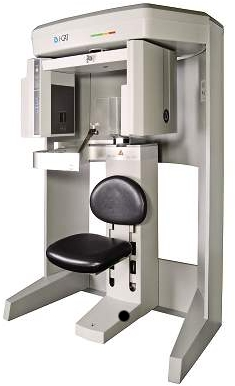
\includegraphics[scale=0.4]{feixe_conico.jpg}
\caption{Tomógrafo odontológico - www.kavo.com.br}
\end{figure}

A aquisição das imagens é feita com o paciente na vertical (ao contrário da tomografia médica,
em que o paciente fica na horizontal). Um emissor e um sensor de raios-X circundam o crânio
do paciente, formando um arco de $180^\circ$ ou $360^\circ$. As imagens geradas pelo tomógrafo
podem ser interpretadas como um volume com o crânio do paciente imerso. Esse volume é "fatiado"
pelo software do aparelho, podendo-se gerar imagens com espaçamentos diferentes ou outros
tipos de imagens, como a visão panorâmica da região de interesse.

As imagens adquiridas por tomógrafos odontológicos costumam exigir um maior pós-processamento
quando é necessário separar (segmentar) determinadas estruturas usando outros softwares como
o InVesalius. Isso ocorre porque, normalmente, essas imagens possuem mais níveis de cinza que
a escala de Hounsfield, o que torna o uso de padrões de segmentação \textit{(presets)} menos
eficiente. Outra característica bastante comum nas imagens provindas de tomógrafos
odontológicos é a alta presença de ruídos do tipo \textit{speckle} e a presença de outros
ruídos normalmente causados por uso de próteses de amálgama pelo paciente.


\subsection{Ressonância Magnética}

A ressonância magnética é um exame realizado sem o uso de radiação ionizante. Em vez disso,
é utilizado um forte campo magnético para alinhar os átomos de algum elemento presente em
nosso corpo, comumente o hidrogênio. Após o alinhamento, são disparadas ondas de rádio, e os
átomos são excitados. Os sensores medem o tempo que os átomos de hidrogênio demoram para se
alinhar novamente. Com isso, é possível determinar qual é o tipo de tecido, pois tecidos
diferentes apresentam quantidades diferentes de átomos de hidrogênio.

Para evitar interferências e melhorar a qualidade do sinal de radiofrequência, além de o
paciente ficar dentro do equipamento, é colocada uma bobina na região de interesse.

 
\begin{figure}[!htb]
\centering
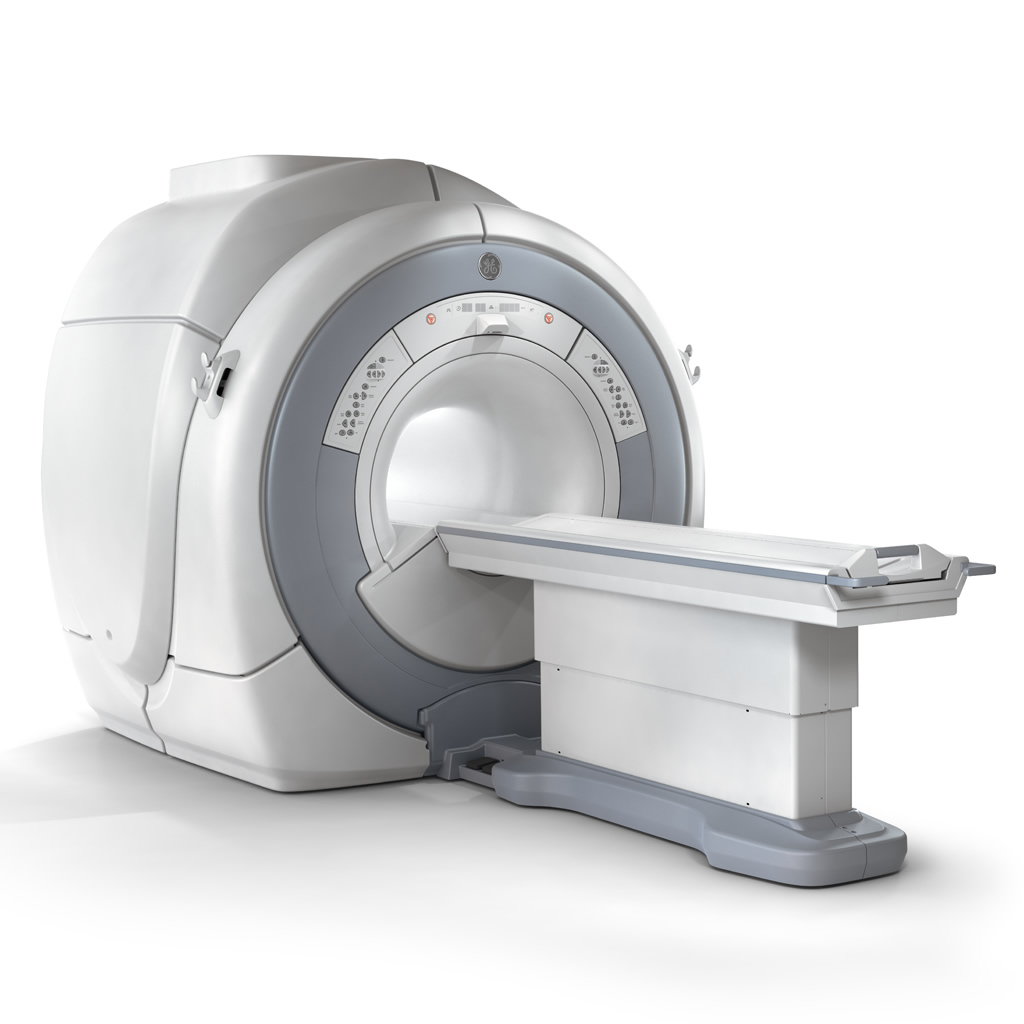
\includegraphics[scale=0.2]{rm_ge.jpg}
\caption{Equipamento de ressonância magnética - www.gehealthcare.com}
\end{figure}

\begin{figure}[!htb]
\centering
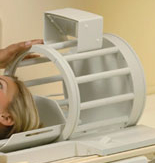
\includegraphics[scale=0.8]{bobina.jpg}
\caption{Bobina - www.healthcare.philips.com}
\end{figure}

\subsection{Neuronavegação}
\label{sec:neuronavegador_intro}

Neuronavegação é a uma técnica que permite localizar e rastrear instrumentos cirúrgicos em relação às estruturas neuronais através da visualização computacional. Além disso, sistemas de neuronavegação têm sido apontados como uma ferramenta fundamental para estudos em planejamento pré-cirúrgico e aumentar a precisão de experimentos em neurociência, como a estimulação magnética transcraniana (EMT), eletroencefalografia (EEG), magnetoencefalografia (MEG) e espectroscopia no infravermelho próximo. Apesar do vasto campo de aplicações, o uso da neuronavegação em centros de pesquisa é limitado pelo alto custo. O módulo de neuronavegação do InVesalius oferece aos usuários uma alternativa de baixo custo e código aberto aos sistemas comercias de navegação. Desta maneira, é possível utilizar ferramentas específicas para neuronavegação e ainda ter a possibilidade de desenvolvimento de funcionalidades sob demanda. O neuronavegador é distribuído em uma versão executável compatível com sistemas operacionais Windows 7, 8 e 10.. O capítulo~\ref{sec:neuronavegador}, apresenta detalhes sobre o uso desta ferramenta.


\section{Recursos necessários}
O InVesalius é projetado para executar em computadores pessoais, como
\textit{desktops} e \textit{notebooks}. Atualmente, ele é compatível com
os seguintes sistemas operacionais:\\
- MS-Windows (Windows 7, 8 e 10)\\
- GNU/Linux (Ubuntu, Mandriva, Fedora)\\
- Apple Mac OS X

O desempenho do InVesalius depende, principalmente, da quantidade de fatias
reconstruídas (imagens abertas pelo software), da quantidade de memória RAM
disponível, da frequência do processador e da arquitetura do sistema operacional
(32 \textit{bits} ou 64 \textit{bits}).

Vale ressaltar, como regra geral, que quanto maior a quantidade de memória RAM
disponível no sistema, maior será o número de fatias que podem ser abertas
simultaneamente para um dado estudo. Por exemplo, com 1 GB de memória disponível,
pode-se abrir cerca de 300 fatias com resolução de 512x512 \textit{pixels}.
Já com 4 GB de memória, pode-se abrir em torno de 1000 imagens com a mesma
resolução.

			
\subsection{Configurações mínimas}
Sistema Operacional de 32 \textit{bits}\\
Processador Intel Pentium 4 ou equivalente, com frequência de 1,5 GHz\\
1 GB de memória RAM\\
80 GB de disco rígido\\
Placa gráfica com 64 MB de memória\\
Resolução de vídeo de 1024x768 \textit{pixels}


\subsection{Configurações recomendadas}
Sistema Operacional de 64 \textit{bits}\\
Processador Intel Core 2 Duo ou equivalente, com frequência de 2,5 GHz\\
4 GB de memória RAM\\
180 GB de disco rígido\\
Placa gráfica NVidia ou ATI, com 128 MB de memória\\
Resolução de vídeo de 1024x768 \textit{pixels}


\chapter{Installation}

\section{MS-Windows}


To install InVesalius on MS-Windows, simply run the installer program. When a window asking you to confirm the file execution appears, click \textbf{Yes}.

\begin{figure}[!htb]
\centering
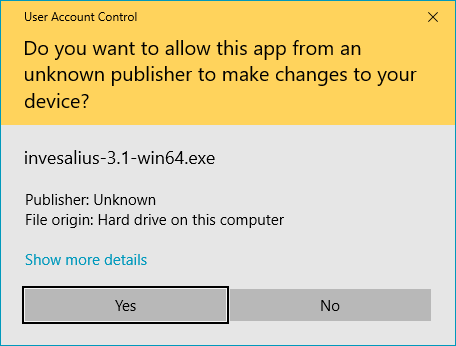
\includegraphics[scale=0.5]{installation_exec_en.png}
\end{figure}

\newpage

A new window will ask you to select the language of the installer. Select the language and click \textbf{OK} button.

\begin{figure}[!htb]
\centering
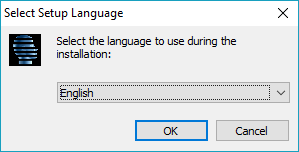
\includegraphics[scale=0.7]{installation_select_language_en.png}
\end{figure}
 
\hspace{.2cm}

Window installer appears. Click \textbf{Next}.


\begin{figure}[!htb]
\centering
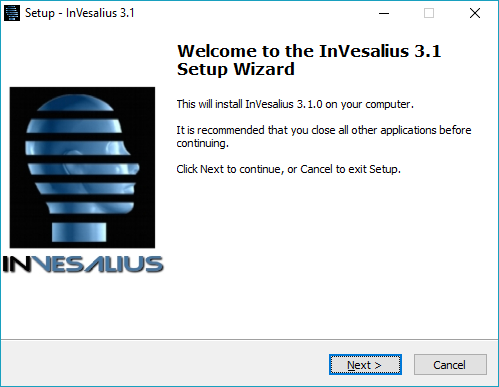
\includegraphics[scale=0.7]{installation_welcome_en.png}
\end{figure}

\newpage

Select \textbf{I accept the agreement} and click on \textbf{Next} button.

\begin{figure}[!htb] 
\centering
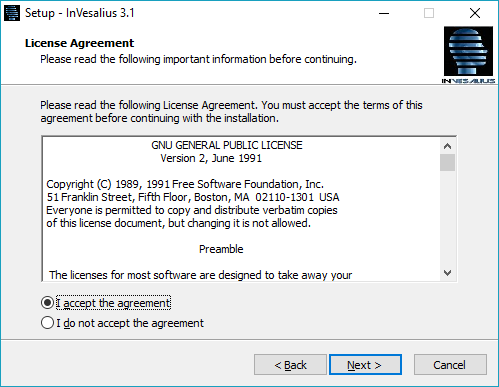
\includegraphics[scale=0.7]{installation_license_en.png}
\end{figure}

\hspace{.2cm}

Click on \textbf{Next} button again. 

\begin{figure}[!htb]  
\centering
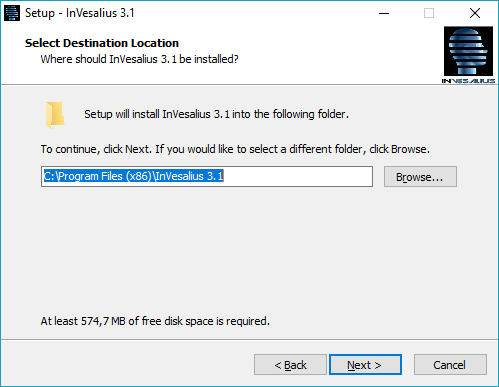
\includegraphics[scale=0.7]{installation_folder_en.png}
\end{figure}

\newpage

Click on \textbf{Next}  button.
\begin{figure}[!htb]
\centering
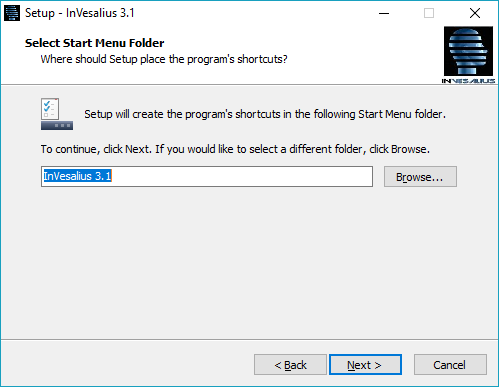
\includegraphics[scale=0.7]{installation_program_name_en.png}
\end{figure}

\hspace{.2cm}

Select \textbf{Create a desktop shortchut} and click on \textbf{Next}.

\begin{figure}[!htb]
\centering
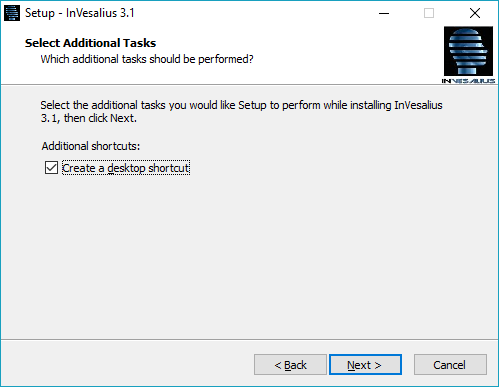
\includegraphics[scale=0.7]{installation_desktop_shortcut_en.png}
\end{figure}

\newpage

Click on \textbf{Install} button.

\begin{figure}[!htb]
\centering
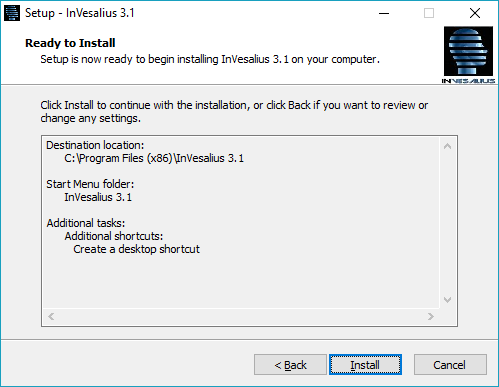
\includegraphics[scale=0.7]{installation_resume_en.png}
\end{figure}

\hspace{.2cm}

While the software is installed, a progress window will appear.

\begin{figure}[!htb]
\centering
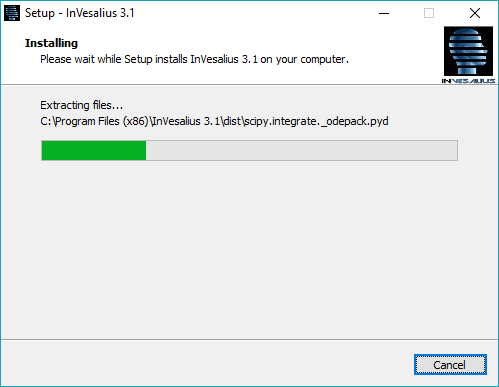
\includegraphics[scale=0.7]{installation_progress_en.png}
\end{figure}

\newpage

To run InVesalius after installation, check \textbf{Lauch InVesalius 3.1} and click on \textbf{Finish} button.

\begin{figure}[!htb]
\centering
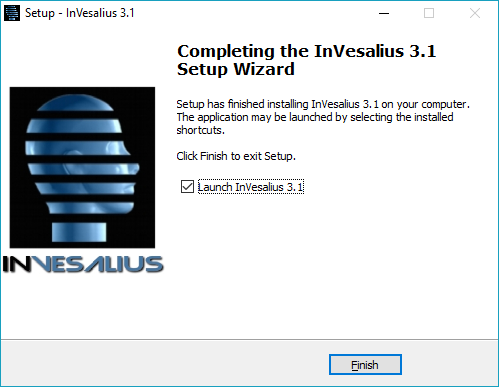
\includegraphics[scale=0.7]{installation_finish_en.png}
\end{figure}

\hspace{.2cm}

If this is the first time the software is installed, a window will appear to select the InVesalius language. Select the language you want and click on \textbf{OK} button.

\begin{figure}[!htb]
\centering
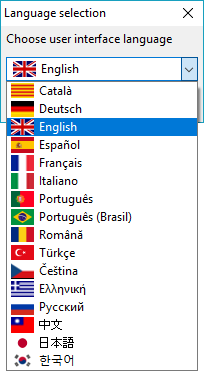
\includegraphics[scale=0.6]{invesalius_language_select_en.png}
\end{figure}

\newpage

While InVesalius is loaded, an opening window like the one in the next figure is displayed.

\begin{figure}[!htb]
\centering
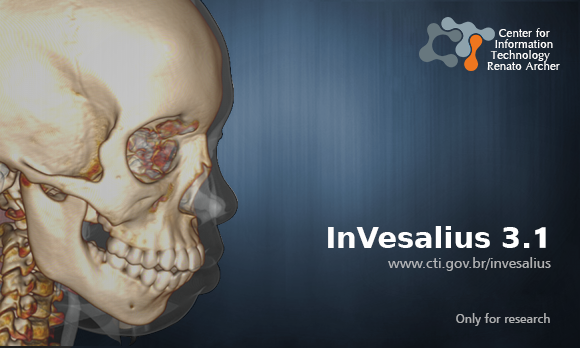
\includegraphics[scale=0.4]{splash_en.png}
\end{figure}

\hspace{.2cm}

Then, the main program window open.

\begin{figure}[!htb]
\centering
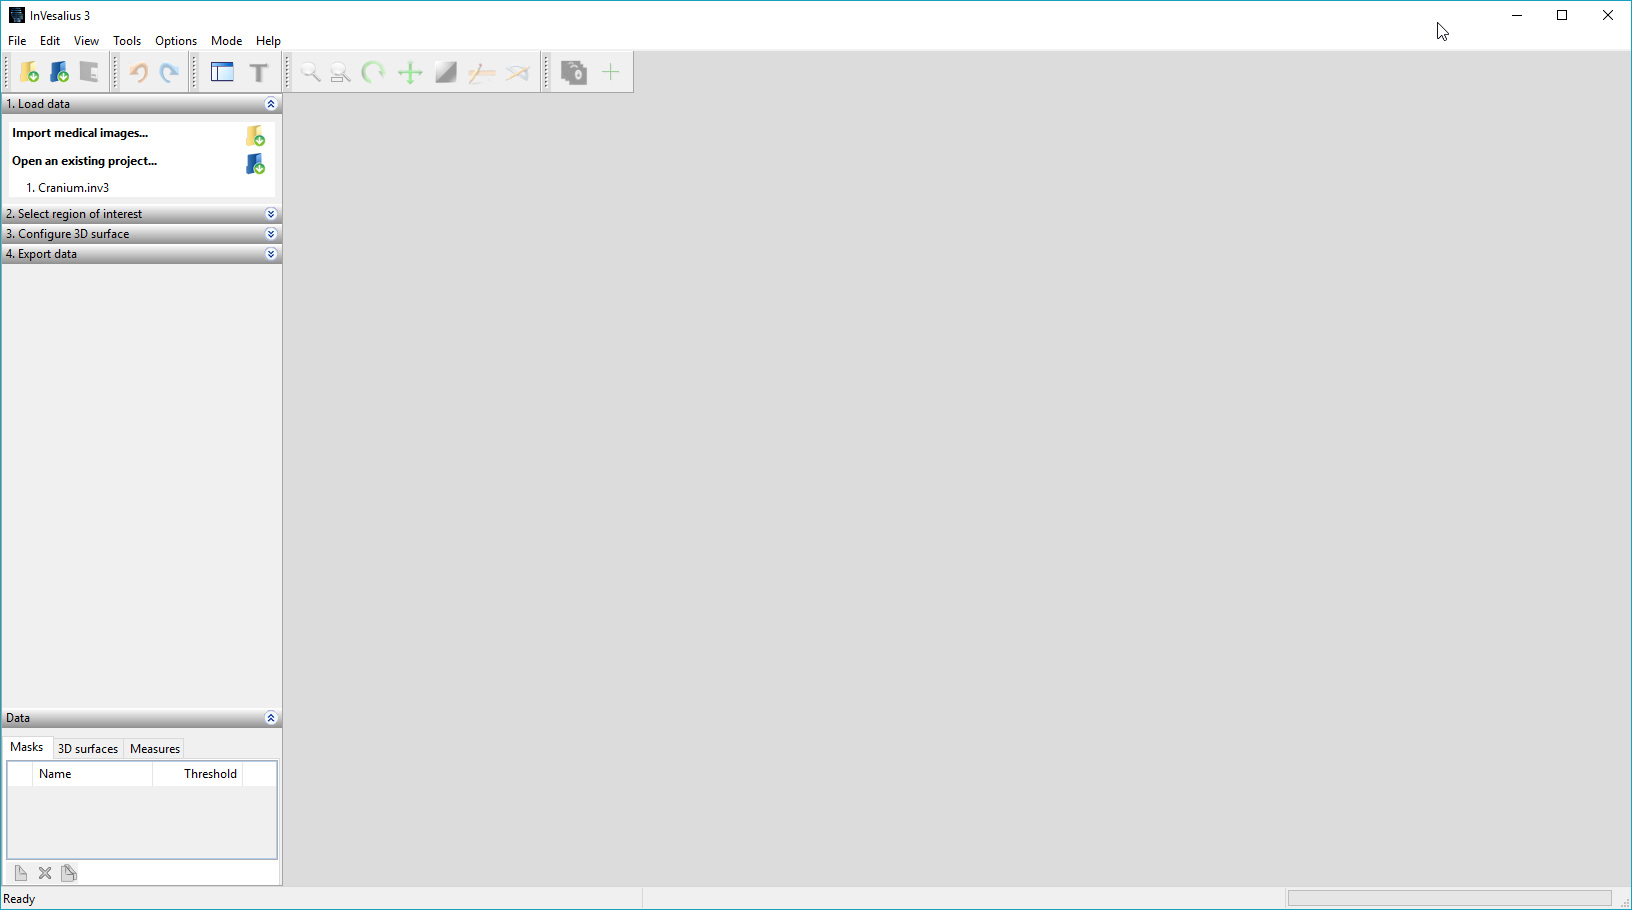
\includegraphics[scale=0.3]{main_window_without_project_en.png}
\end{figure}

\section{Mac Os X}

To start the installation on Mac Os X, double-click the installer with the left mouse button.
Then the installer will be initialized.

\begin{figure}[!htb]
\centering
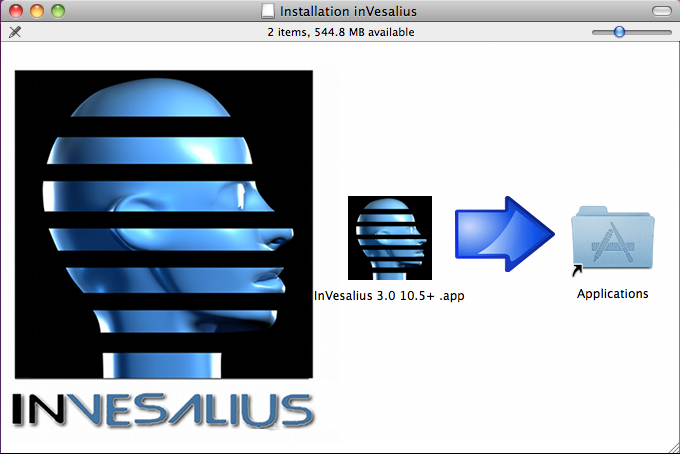
\includegraphics[scale=0.3]{mac2.png}
\end{figure}

Hold down the left button on the InVesalius software icon and drag it to the \textit{Applications}. Both contained in the installer.

\begin{figure}[!htb]
\centering
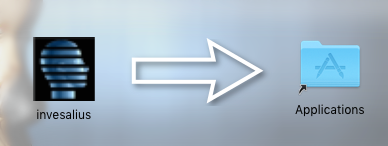
\includegraphics[scale=0.4]{mac4.png}
\end{figure}

The software is already installed, just access through the menu.
\chapter{Image import}

InVesalius imports files in DICOM format, including compressed files (lossless JPEG), Analyze (Mayo Clinic) $^\copyright$, NIfTI, PAR/REC, BMP, TIFF, JPEG and PNG formats.

\section{DICOM}

On menu \textbf{File}, click on \textbf{Import DICOM...}. If you prefer, use the shortcut of keyboard \textbf{Ctrl + I}. Import DICOM images can also be triggered by the toolbar icon described in the figure~\ref{fig:import}.

\begin{figure}[!htb]
\centering

\includegraphics[scale=0.2]{file_import_original.png}
\caption{Shortcut to DICOM import}
\label{fig:import}
\end{figure}

\hspace{.2cm}

Then select the directory containing the DICOM files, as in figure~\ref{fig:win_folder}. InVesalius will search for files also in subdirectories of the chosen directory, if they exist.

\newpage

Click on \textbf{OK} button.

\begin{figure}[!htb]
\centering
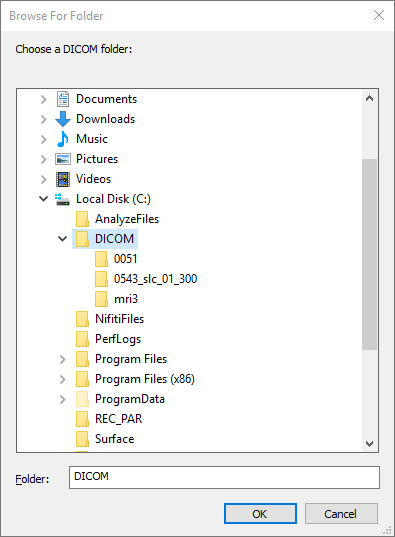
\includegraphics[scale=0.5]{import_select_folder_en.png}
\caption{Folder Selection}
\label{fig:win_folder}
\end{figure}

\hspace{.2cm}

While InVesalius search for DICOM files in the directory, the loading progress of the scanned files is displayed, as shown in the figure~\ref{fig:ver_file}.

\begin{figure}[!htb]
\centering
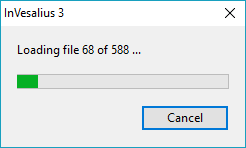
\includegraphics[scale=0.6]{import_load_files_en.png}
\caption{Loading file status}
\label{fig:ver_file}
\end{figure}

\newpage

If DICOM files are found, a window open (figure~\ref{fig:win_import}) to select the patient and the respective series to be opened. It is also possible to skip images for reconstruction.

\begin{figure}[!htb]
\centering
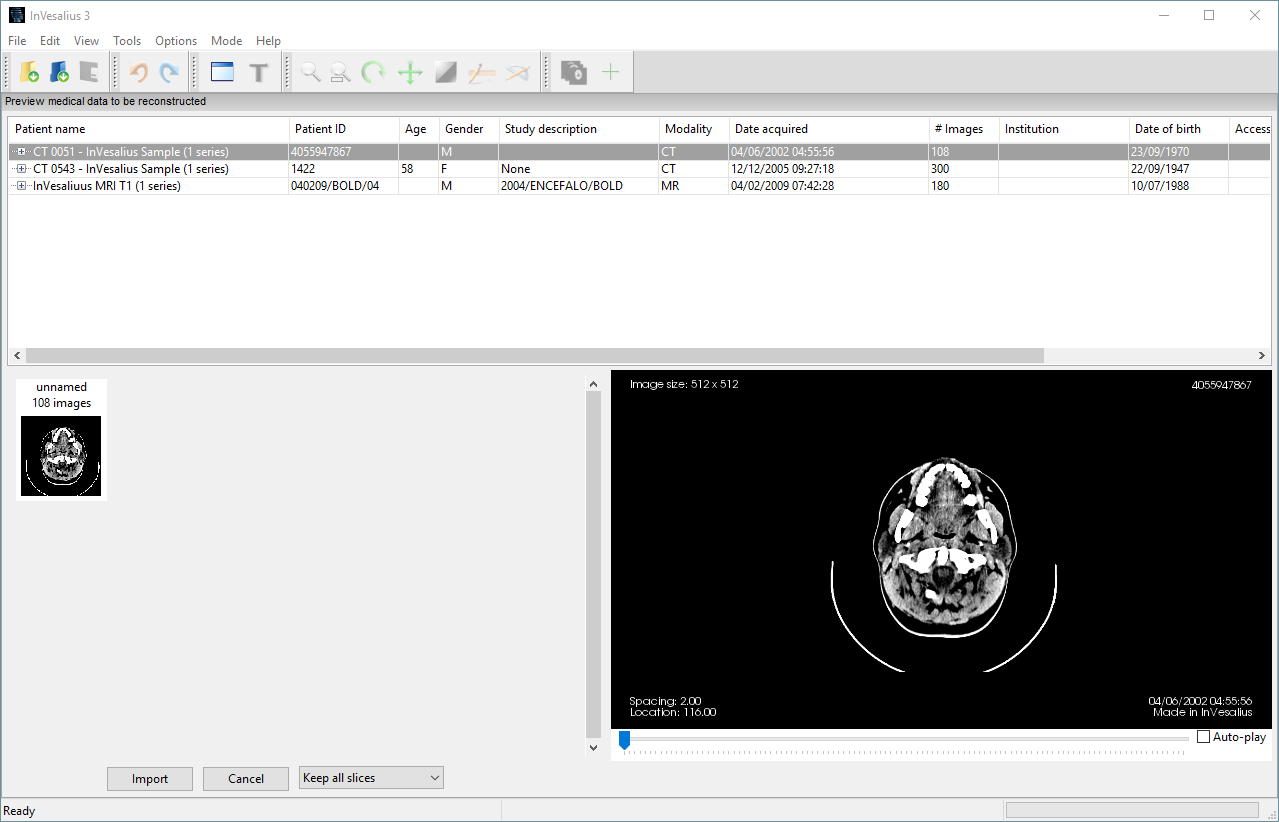
\includegraphics[scale=0.4]{import_window_en.png}
\caption{Import window}
\label{fig:win_import}
\end{figure}

\newpage

If you want to import a series with all the images present, click "\textbf{+}" on the side patient's name to expand the series belonging to him. \textbf {Double-click} with left mouse button on the description of the series. See figure~\ref{fig:import_serie}.

\begin{figure}[!htb]
\centering
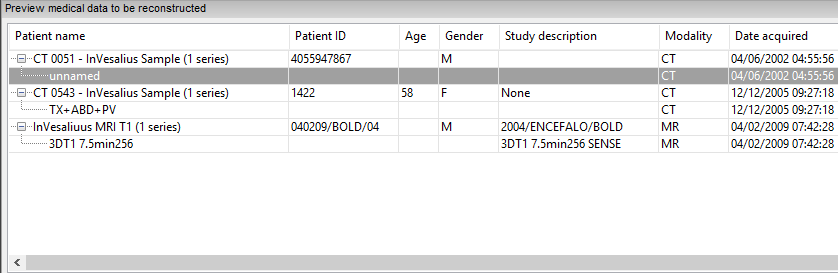
\includegraphics[scale=0.5]{import_window_detail_en.png}
\caption{Series selection}
\label{fig:import_serie}
\end{figure}
 
Some cases in particular when there is no computer with memory and/or satisfactory processing to work with many images in a series, can be it is recommended to skip (skip) some of them. To do this, click \textbf {once} with the \textbf{left} of the mouse over the description of the series (figure~\ref{fig:import_serie}) and select how many images will be skipped (figure~\ref{fig:skip_image}). Click on~\textbf {Import} button.

\begin{figure}[!htb]
\centering
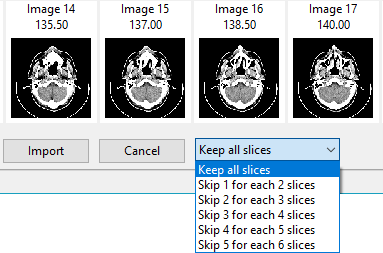
\includegraphics[scale=0.6]{import_window_skip_slice_en.png}
\caption{Skip imagens option}
\label{fig:skip_image}
\end{figure}

If insufficient amount of available memory is detected at the time of loading the images it is recommended reduce the resolution of the slices to work with volumetric and surface visualization, as shown in the \ref{fig:resize_image} window.
The slices will be resized according to the percentage relative to the original resolution. For example, if each slice of the exam contains the dimension of 512 x 512 pixels and the "Percentage of original resolution" is suggested to be 60 \%, each resulting image will be 307 x 307 pixels. If you want to open with the original resolution select the value 100.

\begin{figure}[!htb]
\centering
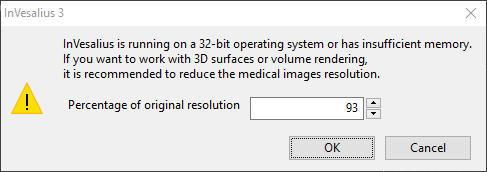
\includegraphics[scale=0.5]{import_window_lower_memory_en.png}
\caption{Image size reduction}
\label{fig:resize_image}
\end{figure}

If the image was obtained with the gantry tilted it will be necessary to do a correction to avoid deformations on the reconstruction. InVesalius allows the user do this correction. When importing an image with the gantry tilted it will be shown a dialog with the degree of tilt (figure~\ref{fig:gantry_tilt}). It is possible to change this value, but it is not recommended. Click on the \textbf{Ok} button to do the correction. If you click on the \textbf{cancel} button the correction will not be done.

\begin{figure}[!htb]
\centering
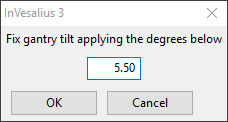
\includegraphics[scale=0.75]{window_gantry_tilt_en.png}
\caption{Gantry tilt correction}
\label{fig:gantry_tilt}
\end{figure}

After the previous procedures, a window will be displayed (figure \ref{fig:prog_recons}) with progress reconstruction (when images are stacked and interpolated).

\begin{figure}[!htb]
\centering
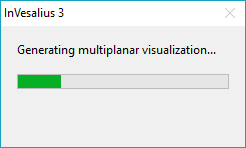
\includegraphics[scale=0.6]{import_window_progress_en.png} 
\caption{Reconstruction progress}
\label{fig:prog_recons}
\end{figure}

\newpage

\section{Analyze}

To import Analyze files, on menu \textbf{File}, click on \textbf{Importar other files...}, then click in the \textbf{Analyze} option as show the figure~\ref{fig:analyze_menu}.

\begin{figure}[!htb]
\centering
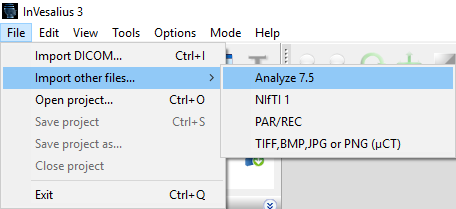
\includegraphics[scale=0.4]{import_analyze_menu_en.png}
\caption{Menu for importing images in analyze format.}
\label{fig:analyze_menu}
\end{figure}

Select the file of Analyze format, in extension \textbf{.hdr} and click on \textbf{Open} button (Figure \ref{fig:analyze_import}).
 
\begin{figure}[!htb]
\centering
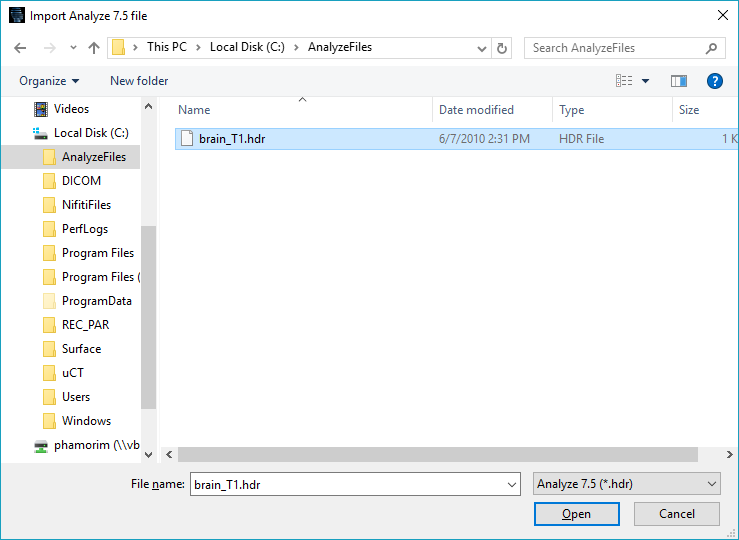
\includegraphics[scale=0.4]{import_analyze_window_en.png}
\caption{Import analyze file format}
\label{fig:analyze_import}
\end{figure}

\section{NIfTI}

To import NIfTI files, on menu \textbf{File}, click on option \textbf{Import other files...} and then click on \textbf{NIfTI} option as shown figure~\ref{fig:import_nifti_menu_pt}.


\begin{figure}[!htb]
\centering
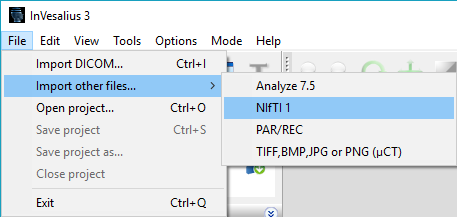
\includegraphics[scale=0.4]{import_nifti_menu_en.png}
\caption{Menu to import images in NIfTI format}
\label{fig:import_nifti_menu_pt}
\end{figure}

Select the file of type NIfTI, on \textbf{nii.gz} or \textbf{.nii} extension, click on \textbf{Open} (figure \ref{fig:import_nifti_window_pt}). If the file is in another extension as \textbf{.hdr}, select \textbf{all files(*.*)} option.

\begin{figure}[!htb]
\centering
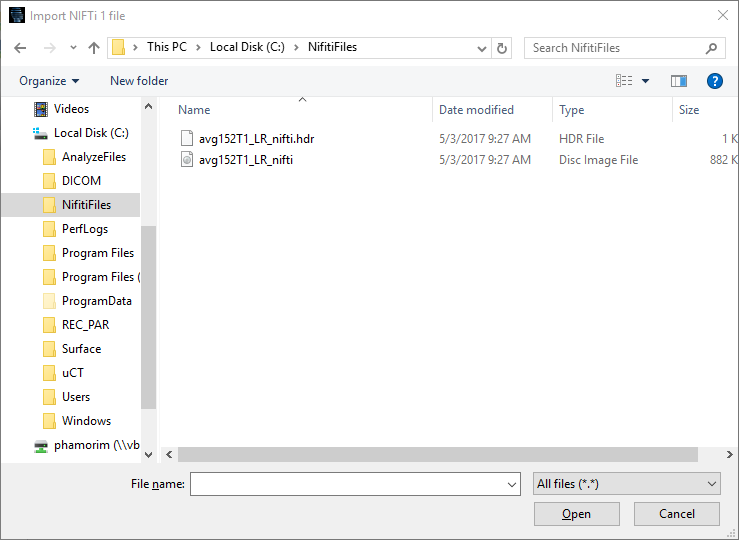
\includegraphics[scale=0.4]{import_nifti_window_en.png}
\caption{Importing images in NIfTI format.}
\label{fig:import_nifti_window_pt}
\end{figure}

\section{PAR/REC}

To import PAR/REC file, on main menu, click on \textbf{File}, \textbf{Import other files...} option and then click on \textbf{PAR/REC} as shown the figure \ref{fig:import_parrec_menu_pt}.

\begin{figure}[!htb]
\centering
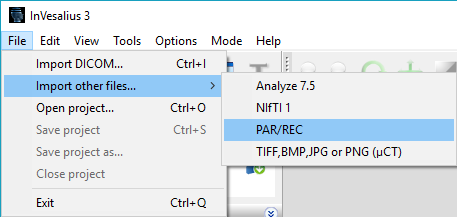
\includegraphics[scale=0.4]{import_parrec_menu_en.png}
\caption{Menu for importing PAR/REC images}
\label{fig:import_parrec_menu_pt}
\end{figure}

Select PAR/REC file type, in extension \textbf{.par} and click on \textbf{Open} (figure~\ref{fig:import_parrec_window_pt}). If the file has no extension, select \textbf{all files(*.*)} option.

\begin{figure}[!htb]
\centering
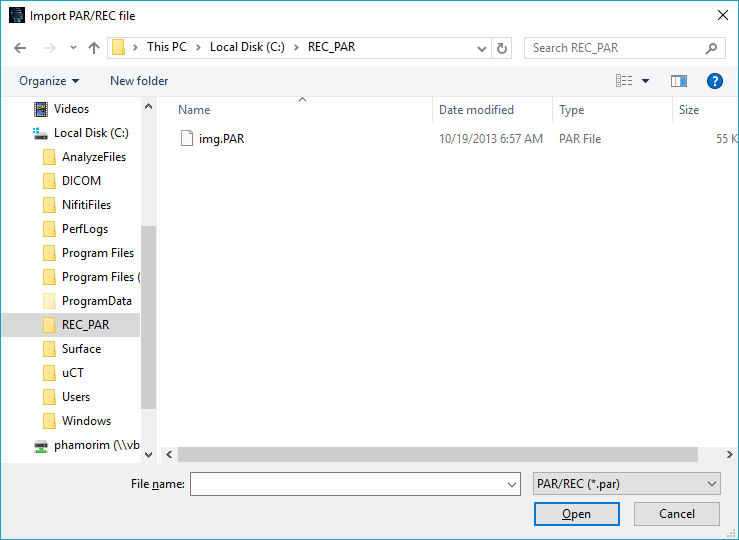
\includegraphics[scale=0.4]{import_parrec_window_en.png}
\caption{PAR/REC import}
\label{fig:import_parrec_window_pt}
\end{figure}

\section{TIFF, JPG, BMP, JPEG or PNG (micro-CT)}

TIFF, JPG, BMP, JPEG or PNG file format for reconstruction can be provided with microtomography equipment (micro-CT or $\mu$CT) or others. InVesalius imports files in these formats if pixels present are represented in \textbf{grayscale}.

To import, click on menu \textbf{File}, \textbf{Import other files...} and then click on \textbf{TIFF, JPG, BMP, JPEG ou PNG ($\mu$CT)} option as shown the figure~\ref{fig:import_bmp_menu_pt}.

\begin{figure}[!htb]
\centering
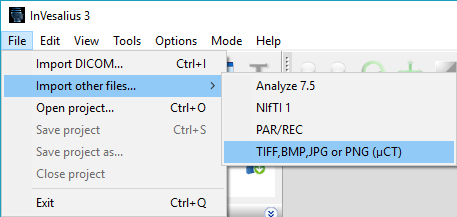
\includegraphics[scale=0.4]{import_bmp_menu_en.png}
\caption{Import images in BMP and others formats}
\label{fig:import_bmp_menu_pt}
\end{figure}

Select the directory that contains the files, as shown the figure~\ref{fig:import_bmp_select_folder}. InVesalius will search for files also in subdirectories of the chosen directory, if they exist. 

Click on \textbf{OK} button.

\begin{figure}[!htb]
\centering
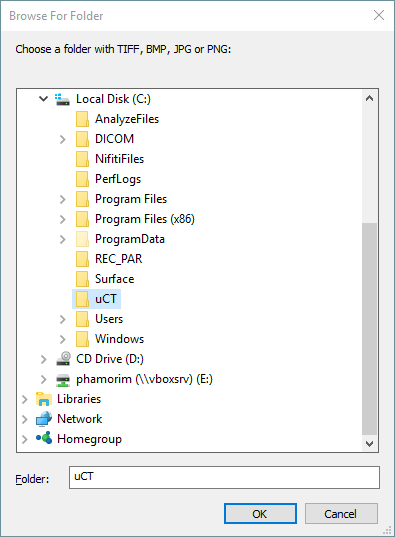
\includegraphics[scale=0.5]{import_bmp_select_folder_en.png}
\caption{Folder selection}
\label{fig:import_bmp_select_folder}
\end{figure}

While InVesalius looking for TIFF, JPG, BMP, JPEG, or PNG files in the directory, the upload progress of the scanned files is displayed, as illustrated by the \ref{fig:import_bmp_load_pt} figure.

\begin{figure}[!htb]
\centering
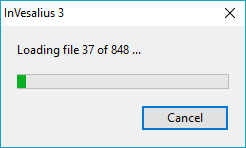
\includegraphics[scale=0.6]{import_bmp_load_en.png}
\caption{Checking and loading files status.}
\label{fig:import_bmp_load_pt}
\end{figure}

If files of type TIFF, JPG, BMP, JPEG or PNG are founded, a window open (figure~\ref{fig:import_bmp_window_pt}) to display the founded files eligible for reconstruction. You can also skip images to rebuild or remove files from the rebuild list. The files are sorted according to the file name, it is recommended to use numbers in their names according to the order you want to get in the rebuild.

\begin{figure}[!htb]
\centering
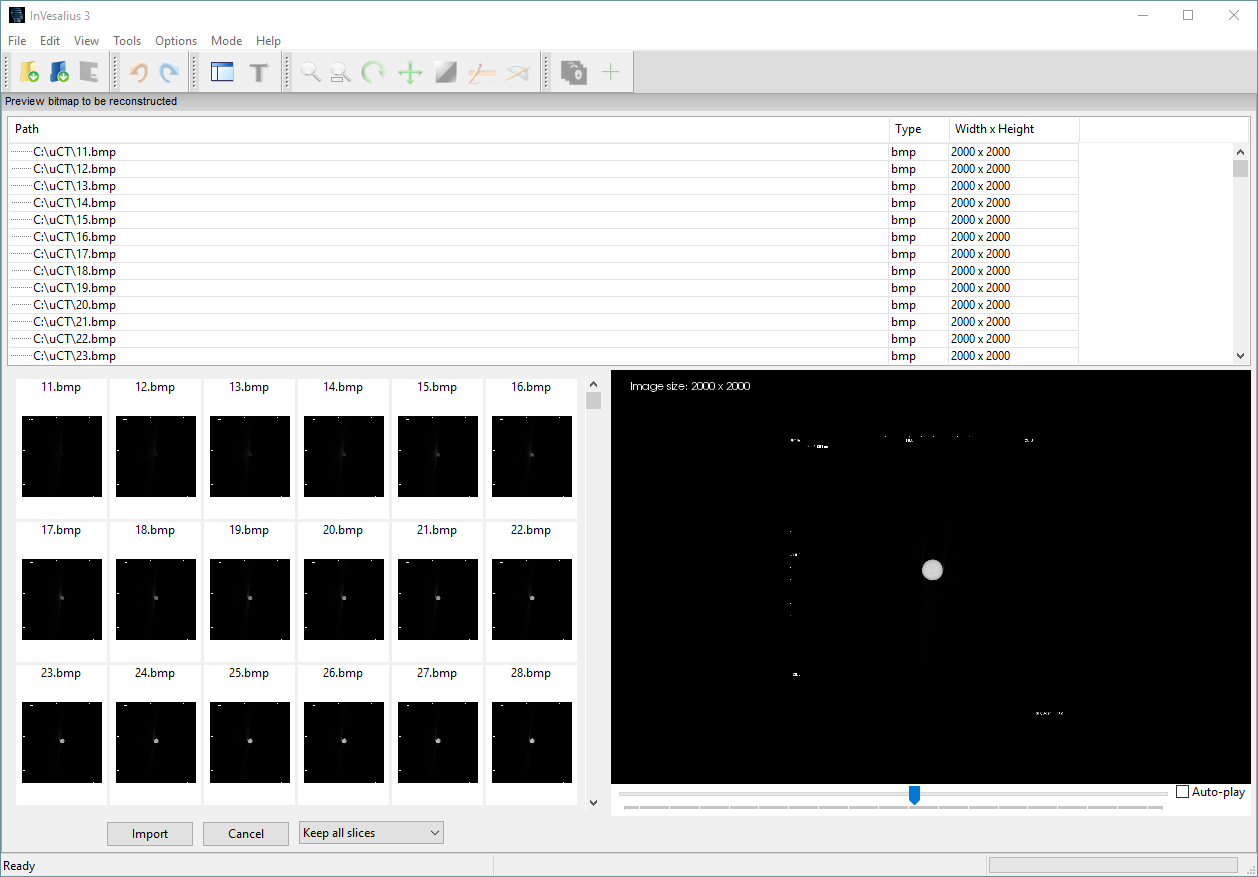
\includegraphics[scale=0.3]{import_bmp_window_en.png}
\caption{Window to import BMP files.}
\label{fig:import_bmp_window_pt}
\end{figure}
 
To delete files that are not of interest, you can select a file by clicking the \textbf{left mouse button} and then pressing the \textbf{delete} key. You can also choose a range of files to delete, so you need to click the \textbf{left mouse button} on the first file in the track, hold down the \textbf{shift} key, click again with the \textbf{button Left mouse button} in the last file of the track and finally press the \textbf{delete} button.
 
Like importing DICOM files module, you can skip BMP images for rebuilding. In some cases, particularly where a computer with satisfactory memory and/or processing is not available to work with many images in a series, it may be advisable to skip (skip) some of them. To do this, select how many images to skip (figure~\ref{fig:import_bmp_skip_pt}). Click \textbf{Import} button.

\begin{figure}[!htb]
\centering
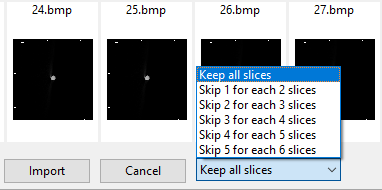
\includegraphics[scale=0.4]{import_bmp_skip_en.png}
\caption{Importation window}
\label{fig:import_bmp_skip_pt}
\end{figure}

To reconstruct this file type, it is necessary to define a name for the project, to indicate the orientation of the images (axial, coronal or sagittal), voxel spacing ($X$, $Y$ and $Z$) in \textbf{mm} as shown in the figure~\ref{fig:import_bmp_spacing_pt}. The voxel spacing in $X$ is the pixel width of each image, $Y$ the pixel length, and $Z$ represents the distance of each slice (voxel height).

If the image set consists of microtomography images, more specifically GE and Brucker equipment, it is possible that InVesalius will read the text file with the acquisition parameters that normally stay in the same folder as the images and automatically insert the spacing . This verification can be done when the values of $X$, $Y$ and $Z$ are different from "1.00000000", otherwise it is necessary to enter the values of the respective spacing.

\textbf{Attention, the spacing is a paramount parameter for the correct dimension of the objects in the software. Incorrect spacing will provide incorrect measurements.}

Once you have completed all the parameters, just click the \textbf{Ok} button.

\begin{figure}[!htb]
\centering
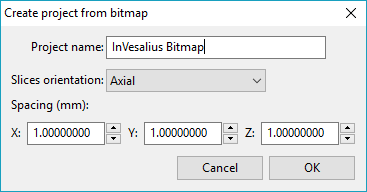
\includegraphics[scale=0.5]{import_bmp_spacing_en.png}
\caption{Tela de importação}
\label{fig:import_bmp_spacing_pt}
\end{figure}

If insufficient memory is available when loading images, it is recommended to reduce the resolution of the slices to work with volumetric and surface visualization, as shown in the \ref{fig:import_bmp_resize_pt} window. The slices will be resized according to the percentage relative to the original resolution. For example, if each slice of the exam contains the dimension of 512 x 512 pixels and the "Percentage of the original resolution" is suggested at 60\%, each resulting image will have 307 x 307 pixels. If you want to open with the original resolution select the value 100.

\begin{figure}[!htb]
\centering
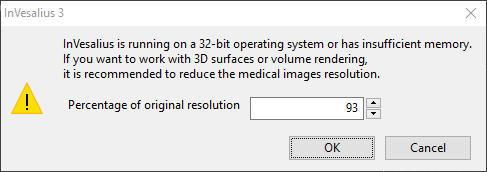
\includegraphics[scale=0.5]{import_window_lower_memory_en.png}
\caption{Image resize}
\label{fig:import_bmp_resize_pt}
\end{figure}

%Após os passos anteriores é necessário aguardar um instante para completar a reconstrução multiplanar conforme mostra a figura~\ref{fig:import_bmp_mpr_pt.png}.

After the previous steps it is necessary to wait a moment to complete the multiplanar reconstruction as shown in the figure~\ref{fig:import_bmp_mpr_pt.png}.

\begin{figure}[!htb]
\centering
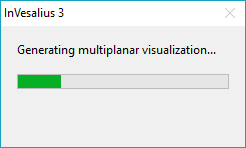
\includegraphics[scale=0.6]{import_window_progress_en.png}
\caption{Multiplanar reconstruction in progress.}
\label{fig:import_bmp_mpr_pt.png}
\end{figure}

\chapter{Image adjustment}

InVesalius does not guarantee the correct image order because sometimes these images have wrong information or do not follow the DICOM standard. Therefore, it is recommended to check if a lesion or an anatomical mark is on the correct side. If not, it is possible to use the flip image or swap axes tools. For image alignment, the rotation image tool can be used.

It is possible to mirror the image, making them flip. To perform that, it is necessary to click in menu, \textbf{Tools}, \textbf{Image}, \textbf{Flip} and click in one of the following options (figure~\ref{fig:menu_img_mirroring_axis_pt}):

\begin{itemize}
	\item Right - Left
	\item Anterior - Posterior
	\item Top - Botton
\end{itemize}

\begin{figure}[!htb]
\centering
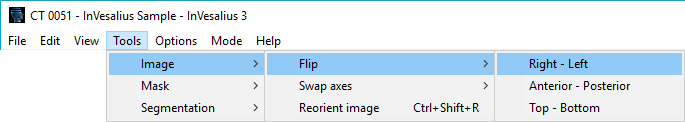
\includegraphics[scale=0.4]{menu_img_mirroring_axis_en.png}
\caption{Menu to activate flip image tool.}
\label{fig:menu_img_mirroring_axis_pt}
\end{figure}


The figure~\ref{fig:mirrored} shows a comparative between the image without being flipped and the flipped image. Due to all image form the volume, if the flip is applied all other orientation are also modified.

\begin{figure}[!htb]
  \centering
  \subfloat[Input image]{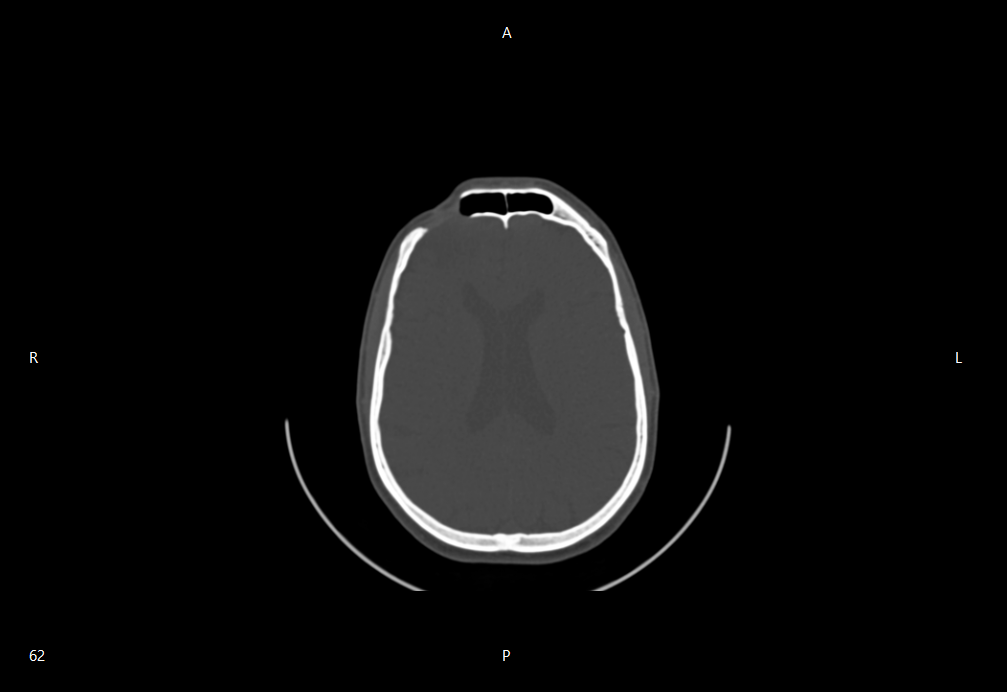
\includegraphics[width=0.45\textwidth]{mirror_axial_en.png}}  \qquad
  \subfloat[Flipped image]{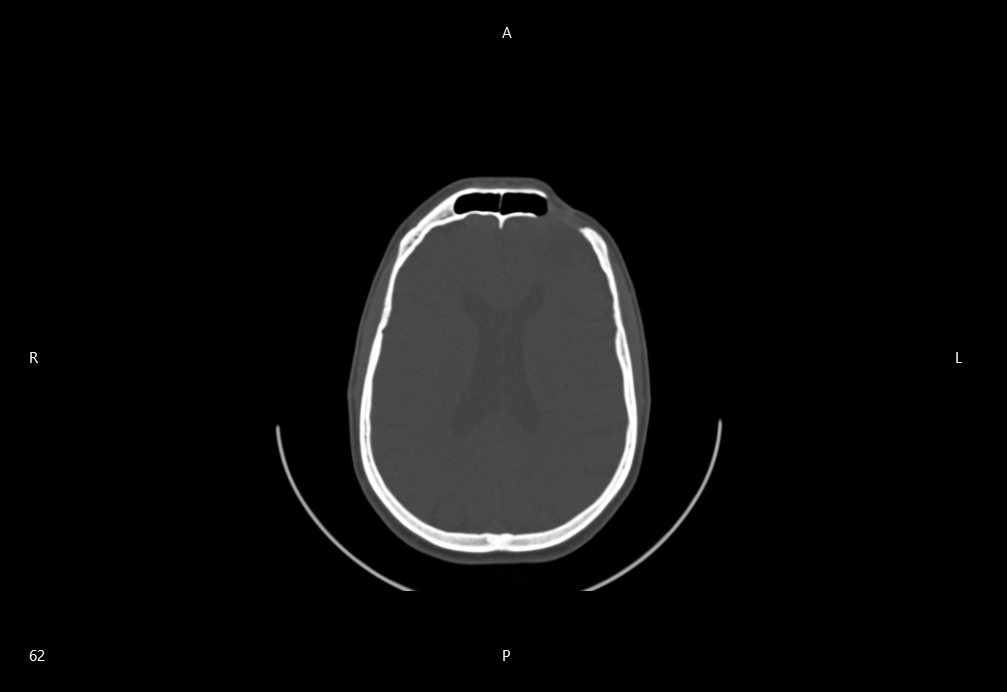
\includegraphics[width=0.45\textwidth]{mirror_axial_mirrored_en.png}}
  \hfill
  \caption{Example of a right-left flipped image.}
  \label{fig:mirrored}
\end{figure}

\section{Swap axes}

The swap axes tool changes the image orientation, in the case that the image has been wrongly imported. To perform that, it is necessary to click in menu, \textbf{Tools}, \textbf{Image}, \textbf{Swap axes} and click in one of the following options (figure~\ref{fig:menu_invert_axis}):

\begin{itemize}
	\item From Right-Left to Anterior-Posterior
	\item From Right-Left to Top-Bottom
	\item From Anterior-Posterior to Top-Bottom
\end{itemize}


The figures~\ref{fig:invert_axis_axial} e~\ref{fig:invert_axis_axial_inverted}, shows an example of images with inverted axis.

\begin{figure}[!htb]
\centering
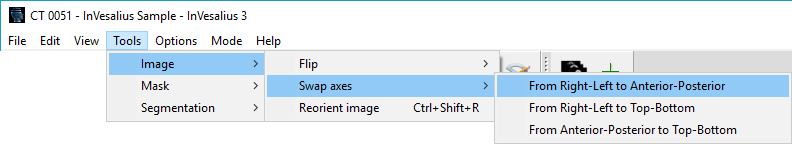
\includegraphics[scale=0.4]{menu_invert_axis_en.png}
\caption{Menu to activate swap image tool.}
\label{fig:menu_invert_axis}
\end{figure}

\begin{figure}[!htb]
\centering
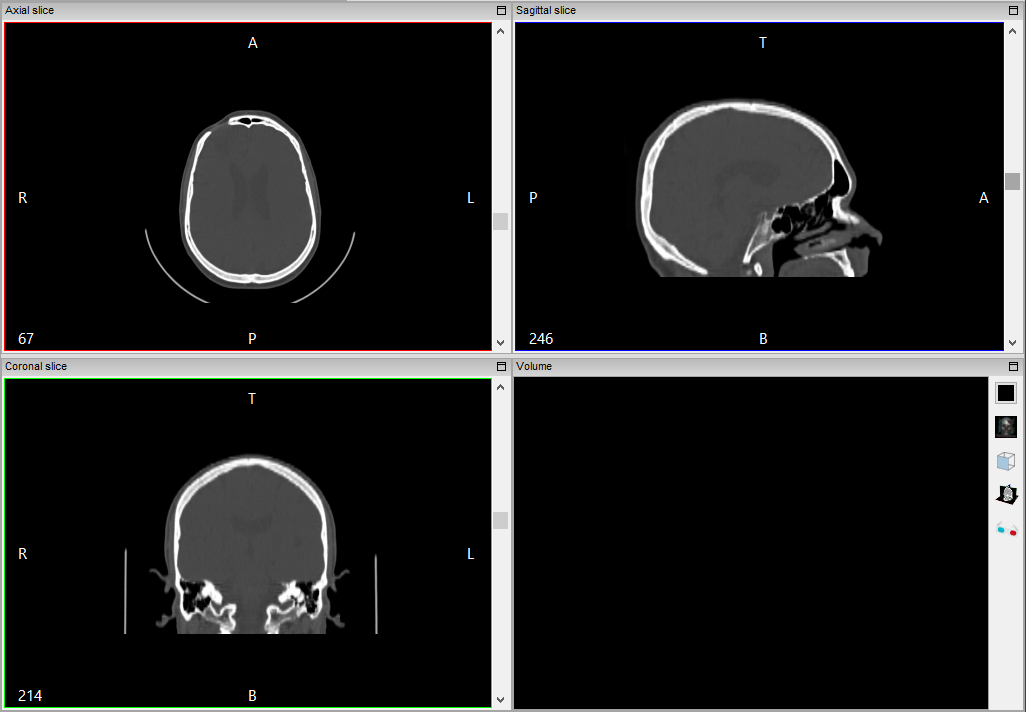
\includegraphics[scale=0.4]{invert_axis_axial_en.png}
\caption{Images before swap axes - from Anterior-Posterior to Top-Bottom.}
\label{fig:invert_axis_axial}
\end{figure}

\begin{figure}[!htb]
\centering
\includegraphics[scale=0.4]{invert_axis_axial_inverted_en.png}
\caption{Images after swap axes - from Anterior-Posterior to Top-Bottom.}
\label{fig:invert_axis_axial_inverted}
\end{figure}

\section{Reorient image (Rotate)}

If it is necessary to align the image taking in account some reference point, e.g. anatomical marker, it is possible by using the reorient image tool. To open this tool it is necessary to click in menu, \textbf{Tools}, \textbf{Image} and \textbf{Reorient image} (figure~\ref{fig:menu_img_reorient}).

\begin{figure}[!htb]
\centering
\includegraphics[scale=0.4]{menu_img_reorient_en.png}
\caption{Menu to activate reorient image tool.}
\label{fig:menu_img_reorient}
\end{figure}

When this tool is activated a window is opened(figure~\ref{fig:image_reorient_window}) that shows which orientation and how much degrees the image was rotated.
\begin{figure}[!htb]
\centering
\includegraphics[scale=0.4]{image_reorient_window_en.png}
\caption{Window that shows the reorientation image parameters.}
\label{fig:image_reorient_window}
\end{figure}

Initially, it is necessary to define the rotation point, to perfom that \textbf{keep the left mouse button pressed} between the two lines intersection (figure~\ref{fig:image_reorient_adjust_center}) at one orientation window, e.g. axial, coronal or sagittal, and drag to the desired point.

\begin{figure}[!htb]
\centering
\includegraphics[scale=0.4]{image_reorient_adjust_center_en.png}
\caption{Defining the axis of rotation of the image.}
\label{fig:image_reorient_adjust_center}
\end{figure}

To rotate the image it is necessary to \textbf{keep the left mouse button pressed} and \textbf{drag} until the reference point or anatomical marker stays align with one of the lines (figure~\ref{fig:image_reorient_rotated}). After the image is in the desired position, it is necessary to click the button \textbf{Apply}, in the parameter window (figure~\ref{fig:image_reorient_window}). This task can take some seconds, depends on the image size. The figure~\ref{fig:image_reorient_rotated_applied} shows an image with reorient done.

\begin{figure}[!htb]
\centering
\includegraphics[scale=0.4]{image_reorient_rotated_en.png}
\caption{Rotated image.}
\label{fig:image_reorient_rotated}
\end{figure}

\begin{figure}[!htb]
\centering
\includegraphics[scale=0.4]{image_reorient_rotated_applied_en.png}
\caption{Rotated image after reorientation is done.}
\label{fig:image_reorient_rotated_applied}
\end{figure}

\chapter{Image Manipulation (2D)}

\section{Multiplanar Reconstruction}

When images are imported, InVesalius automatically shows its reconstruction
Multiplanar in the Axial, Sagittal and Coronal orientations, as well as a window for 3D manipulation.
See figure \ref{fig:mpr}.

\begin{figure}[!htb]
\centering
\includegraphics[scale=0.40]{multiplanar_mask_window_en.png}
\caption{Multiplanar Reconstruction}
\label{fig:mpr}
\end{figure}

\newpage

In addition to creating a multiplanar reconstruction, InVesalius segments an image, highlighting, for example, soft tissue bones. The highlight is represented by the application of colors on a segmented structure, i.e., the colors forms a mask over an image highlighting the structure (figure \ref{fig:mpr}). This is discussed in more detail in the following chapters.


To hide the mask, use the data manager, located in the lower left corner
of the screen. Just choose the tab \textbf{Masks} and click \textbf{once} using the
\textbf{left} mouse buttom over the eye icon next to \textbf{"Mask 1"}. See figure
\ref{fig:ger_masc}.

\begin{figure}[!htb]
\centering
\includegraphics[scale=0.8]{data_mask_en.png}
\caption{Mask manager}
\label{fig:ger_masc}
\end{figure}

The eye icon disappears, and the colors of the segmentation mask are hidden (figure
\ref{fig:mpr_sem_mask}).

\begin{figure}[!htb]
\centering
\includegraphics[scale=0.30]{multiplanar_window_en.png}
\caption{Multiplanar reconstruction without segmentation mask}
\label{fig:mpr_sem_mask}
\end{figure}

\subsection{Axial orientation}

The axial orientation consists of cuts made transversal in relation to the region of interest, i.e. parallel cuts to the axial plane of the human body.
In figure \ref{fig:axial_corte}, an axial image of the skull region is displayed.

\begin{figure}[!htb]
\centering
\includegraphics[scale=0.30]{axial_en.png}
\caption{Axial slice}
\label{fig:axial_corte}
\end{figure}

\subsection{Sagittal orientation}

The sagittal orientation consists of cuts made laterally in relation to the region of interest, i.e. parallel cuts to the sagittal plane of the human body, which divides it into the left and right portions.
In figure \ref{fig:sagital_slice}, a sagittal skull image is displayed.

\begin{figure}[!htb]
\centering
\includegraphics[scale=0.30]{sagital_en.png}
\caption{Sagittal slice}
\label{fig:sagital_slice}
\end{figure}

\newpage

\subsection{Coronal orientation}

The coronal orientation is composed of cuts parallel to the coronal plane, which divides the human body into ventral and dorsal halves.
In figure \ref{fig:coronal_slice} is displayed  a skull image in coronal orientation.

\begin{figure}[!htb]
\centering
\includegraphics[scale=0.30]{coronal_en.png}
\caption{Coronal slice}
\label{fig:coronal_slice}
\end{figure}


\section{Correspondence between the axial, sagittal and coronal orientations}
\label{sec:corresp_all_orient}

To find out the common point of the images in differents orientations, simply activate the "Slices cross intersection" feature with the shortcut icon located on the toolbar.
See figure \ref{fig:cross_icon}.

\begin{figure}[!htb]
\centering
\includegraphics[scale=1]{cross.png}
\caption{Shortcut to show common point between different orientations}
\label{fig:cross_icon}
\end{figure}

When the feature is fired, two cross segments that intersect perpendicularly are displayed on each image (figure \ref{fig:cross_all}). The intersection point of each pair of segments represents the common point between differents orientations.

\newpage

To modify the point, keep \textbf{pressed} the \textbf{left} mouse button and
\textbf{drag}. Automatically, the corresponding points will be updated in each image.

\begin{figure}[!htb]
\centering
\includegraphics[scale=0.4]{multiplanar_window_cross_en.png}
\caption{Common point between differents orientations}
\label{fig:cross_all}
\end{figure}

To disable the feature, simply click on the shortcut again (figure \ref{fig:cross_icon}). This feature can be used in conjunction with the slice editor (which will be discussed later).

\section{Interpolation}

By default the 2D images visualization are interpolated (figure~\ref{fig:interp}).a, to deactivate this feature, in menu press \textbf{View}, \textbf{Interpolated slices} (figure~\ref{fig:menu_interpoleted_image_pt}). In this way it will be possible to visualize each pixel individually as shown in the figure~\ref{fig:interp}.b.

\textbf{Note: This interpolation is for visualization purposes only, not directly influencing segmentation or 3D surface generation.}

\begin{figure}[!htb]
\centering
\includegraphics[scale=0.7]{menu_interpoleted_image_en.png}
\caption{Menu to disable and enable interpolation}
\label{fig:menu_interpoleted_image_pt}
\end{figure}


\begin{figure}[!htb]
  \centering
  \subfloat[Interpolated]{\includegraphics[width=0.4\textwidth]{axial_interpoleted.png}}  \qquad
  \subfloat[Non-interpolated]{\includegraphics[width=0.4\textwidth]{axial_not_interpoleted.png}}
  \hfill
  \caption{Interpolated and non-interpolated image visualization.}
  \label{fig:interp}
\end{figure}

\section{Move}

To move an image on the screen, the toolbar's "Move" shortcut icon can be used (figure
\ref{fig:move_icon}). Click on the icon to activate the feature and then with the \textbf{left} mouse button on the image, \textbf{drag} it to the desired direction. The figure \ref{fig:move_img} shows a displaced (moved) image.

\begin{figure}[!htb]
\centering
\includegraphics[scale=0.25]{tool_translate_original.png}
\caption{Shortcut to move images}
\label{fig:move_icon}
\end{figure}

\begin{figure}[!htb]
\centering
\includegraphics[scale=0.25]{axial_pan_en.png}
\caption{Displaced image}
\label{fig:move_img}
\end{figure}

\section{Rotate}

The image rotation can be activated by the toolbar's "Rotate" shortcut icon (figure \ref{fig:rot_icon}). To rotate an image, click on the icon and then with the \textbf{left} mouse button press on the image, \textbf{drag} clockwise or anticlockwise, depending on the desired direction of rotation.

\begin{figure}[!htb]
\centering
\includegraphics[scale=0.25]{tool_rotate_original.png}
\caption{Shortcut to rotate images}
\label{fig:rot_icon}
\end{figure}

\begin{figure}[!htb]
\centering
\includegraphics[scale=0.25]{axial_rotate_en.png}
\caption{Rotated image}
\label{fig:rotate_all}
\end{figure}

\section{Zoom}

In InVesalius, there are different ways to enlarge an image. You can maximize the desired orientation window, apply zoom directly to the image, or select the region of the image to enlarge.

\subsection{Maximizing orientation windows}

As we already know, the main InVesalius window is divided into 4 subwindows: axial, sagittal, coronal and 3D. Each of these can be maximized to occupy the entire area of the main window. To do this, simply \textbf{left} mouse click on the subwindow icon located in the \textbf{upper right corner} (figure \ref{fig:maximize_window}). To restore a maximized window to its previous size, simply click the icon again.

\begin{figure}[!htb]
\centering
\includegraphics[scale=0.6]{maximize_sagital_mpr.png}
\caption{Detail of a sub-window (Note the maximize icon in the upper right corner)}
\label{fig:maximize_window}
\end{figure}

\subsection{Enlarging or reducing an image}

To enlarging or reducing an image, click on the zoom shortcut icon in the toolbar (figure \ref{fig:zoom_icon}). Hold down the \textbf{left} mouse button on the image and \textbf{drag} the mouse to \textbf{top} if you want to enlarge it, or \textbf{down}, if you want to reduce it.

\begin{figure}[!htb]
\centering
\includegraphics[scale=0.25]{tool_zoom_original.png}
\caption{Zoom shortcut}
\label{fig:zoom_icon}
\end{figure}

%\begin{figure}[!htb]
%\centering
%\includegraphics[scale=0.2]{ScreenHunter_76Dec311201_.jpg}
%\caption{Imagem com \textit{Zoom} aplicado}
%\label{fig:zoom_}
%\end{figure}

\subsection{Enlarging an Image Area}

To enlarging a certain image area, click on the "Zoom based on selection" icon in the toolbar (figure \ref{fig:zoom_icon_loc}). Position the mouse pointer at the start position of the selection, click and hold the \textbf{left} mouse button and \textbf{drag} it to the end selection position, forming a rectangle (figure \ref{fig:zoom_select}). Once the left mouse button is released, the zoom operation will be applied to the selected region (figure \ref{fig:zoom_applied}).

\begin{figure}[!htb]
\centering
\includegraphics[scale=0.25]{tool_zoom_select_original.png}
\caption{Zoom based on selection shortcut}
\label{fig:zoom_icon_loc}
\end{figure}

\begin{figure}[!htb]
\centering
\includegraphics[scale=0.25]{tool_zoom_select_image_en.png}
\caption{Area selected for zoom}
\label{fig:zoom_select}
\end{figure}

\begin{figure}[!htb]
\centering
\includegraphics[scale=0.25]{tool_image_with_zoom_en.png}
\caption{Enlarged Image}
\label{fig:zoom_applied}
\end{figure}


\section{Brightness and contrast (Windows)}
\label{sec:ww_wl}

To improve images visualization, the feature \textit{window width} and \textit{window level} can be used, popularly known as "brightness and contrast" or "window" (for radiologists). With this feature, it is possible to set the range of the gray scale (\textit{window level}) and the width of the scale (\textit{window width}) to be used to display the images.

The feature can be triggered by the "Contrast" shortcut icon in the toolbar. See figure \ref{fig:window_level_shortcut}.

\begin{figure}[!htb]
\centering
\includegraphics[scale=0.70]{tool_contrast_original.png}
\caption{Brightness and contrast shortcut}
\label{fig:window_level_shortcut}
\end{figure}

To increase the brightness, hold down the \textbf{left} mouse button and \textbf{drag} horizontally to the right. To decrease the brightness, simply drag the mouse to the left. The contrast can be changed by dragging the mouse (with the \textbf{left} button pressed) vertically: up to increase, or down to decrease the contrast.

To disable the feature, click again on the shortcut icon (figure \ref{fig:window_level_shortcut}).

You can use preset brightness and contrast patterns. The table \ref{tab:window_level} lists some tissues types with their respective brightness and contrast values for the image. To use the presets patterns, position the mouse cursor over the image and \textbf{right-click} to open a context menu on it. When the menu opens, select \textbf{Window width and level}, and then click on the preset option, according to the tissue type, as shown in the figure \ref{fig:window_level}.

\begin{figure}[!htb]
\centering
\includegraphics[scale=0.40]{menu_window_and_level_en.png}
\caption{Context menu for brightness and contrast selection}
\label{fig:window_level}
\end{figure}

\begin{table}[h]
\centering
\caption{Brightness and contrast values for some tissues}
\begin{tabular}{lcc}\\
\hline % este comando coloca uma linha na tabela
Tissue & Brightness & Contrast\\
\hline
\hline
Default & Exam & Exam\\
Manual & Changed & Changed\\
Abdomen & 350 & 50\\
Bone & 2000 & 300\\
Brain & 80 & 40\\
Brain posterior fossa & 120 & 40\\
Contour & 255 & 127\\
Emphysema & 500 & -850\\
Ischemia - Hard, non contrast & 15 & 32\\
Ischemia - Soft, non contrast & 80 & 20\\
Larynx & 180 & 80\\
Liver & 2000 & -500\\
Lung Hard & 1000 & -600\\
Lung Soft & 1600 & -600\\
Mediastinum & 350 & 25\\
Pelvis & 450 & 50\\
Sinus & 4000 & 400\\
Vasculature - Hard & 240 & 80\\
Vasculature - Soft & 680 & 160\\
\hline
\end{tabular}
\label{tab:window_level}
\end{table} 

\newpage

\begin{figure}
  \centering
  \subfloat[Bone]{\label{fig:contrast_bone}\includegraphics[width=0.4\textwidth]{contraste_osso}}
  \subfloat[Lung]{\label{fig:contrast_isq}\includegraphics[width=0.4\textwidth]{contraste_pulmao}}
  \caption{Different types of brightness and contrast}
  \label{fig:two_window_level}
\end{figure}



\section{Pseudo color}

Another feature to improve the visualization of the images is the pseudo color. They replace gray levels by color, or by inverted gray levels. In the latter case, previously clear regions of the image become darker and vice versa.

To change the view using a pseudo color, position the mouse cursor over the image and \textbf{right-click} to open a context menu on it. When the menu opens, select the entry \textbf{Pseudo color}, and then click on the desired pseudo color option, as shown in the figure \ref{fig:pseudo_color}.

\begin{figure}[H]
\centering
\includegraphics[scale=0.40]{pseudo_menu_en.png}
\caption{Pseudo Color}
\label{fig:pseudo_color}
\end{figure}

Figures \ref{fig:image_default} through \ref{fig:image_saturation} exemplify the various pseudo color options available.\\

\begin{figure}[H]
\centering
\includegraphics[scale=0.30]{pseudo_default.jpg}
\caption{Default}
\label{fig:image_default}
\end{figure}

\begin{figure}[H]
\centering
\includegraphics[scale=0.30]{pseudo_inverse.jpg}
\caption{Inverted Gray Image}
\label{fig:image_inverted}
\end{figure}

\begin{figure}[H]
\centering
\includegraphics[scale=0.30]{pseudo_rainbow.jpg}
\caption{Rainbow}
\label{fig:image_arc}
\end{figure}

\begin{figure}[H]
\centering
\includegraphics[scale=0.30]{pseudo_desert.jpg}
\caption{Desert}
\label{fig:image_desert}
\end{figure}

\begin{figure}[H]
\centering
\includegraphics[scale=0.30]{pseudo_hue.jpg}
\caption{Hue}
\label{fig:image_matiz}
\end{figure}

\begin{figure}[H]
\centering
\includegraphics[scale=0.30]{pseudo_ocean.jpg}
\caption{Ocean}
\label{fig:image_ocean}
\end{figure}

\begin{figure}[H]
\centering
\includegraphics[scale=0.30]{pseudo_saturation.jpg}
\caption{Saturation}
\label{fig:image_saturation}
\end{figure}

\newpage

\section{Projection type}

It is possible to change the projection type of the 2D images, in addition to the normal mode, InVesalius has six types of projections that can be accessed as follows: Place the mouse over the image and \textbf{rigth-click} to open a context menu on it. When the menu opens, select the projection type option, and then click on the desired projection option, as shown in the figure ~\ref{fig:menu_proj}.

\begin{figure}[H]
\centering
\includegraphics[scale=0.40]{menu_projection_en.png}
\caption{Projection Type menu}
\label{fig:menu_proj}
\end{figure}

\subsection{Normal}

Normal mode is the default view, i.e. without any type of projection, originally when the image was acquired or customized previously with either brightness and contrast or pseudo color. As shown in figure ~\ref{fig:proj_normal}.

\begin{figure}[H]
\centering
\includegraphics[scale=0.40]{multiplanar_window_en.png}
\caption{Normal projection}
\label{fig:proj_normal}
\end{figure}

\subsection{MaxIP}
\label{sec:max_ip}
MaxIP is also known as MIP (\textit{Maximum Intensity Projection}), the method selects only voxels that have maximum intensity among the visited ones as shown in figure ~\ref{fig:proj_maxip}. According to the amount or "depth" of MaxIP each voxel is visited in order of overlap, for example, to select MaxIP of the pixel $(0,0)$ consisting of 3 slices it is necessary to visit the pixel $(0,0)$ of slices $(1,2,3)$ and select the highest value.

\begin{figure}[H]
\centering
\includegraphics[scale=0.40]{multiplanar_window_maxip_en.png}
\caption{MaxIP projection}
\label{fig:proj_maxip}
\end{figure}

As shown in the figure~\ref{fig:proj_maxip_qtd}, the number of images that will be composed of MaxIP is set at the bottom of each orientation image.

\begin{figure}[H]
\centering
\includegraphics[scale=0.80]{multiplanar_window_maxip_number_en.png}
\caption{Selection the amount of images that composes the MaxIP or MIP}
\label{fig:proj_maxip_qtd}
\end{figure}

\subsection{MinIP}

Unlike MaxIP, MinIP (\textit{Minimun Intensity Projection}) selects only the voxels that have minimal internsity among the visited ones, an example is shown in figure~\ref{fig:proj_minIP}. The image number selection that will compose the projection is made at the bottom of each orientation image as shown in figure~\ref{fig:proj_maxip_qtd}.

\begin{figure}[H]
\centering
\includegraphics[scale=0.40]{multiplanar_window_minip_en.png}
\caption{MinIP projection}
\label{fig:proj_minIP}
\end{figure}

\subsection{MeanIP}
The MeanIP (\textit{Mean Intensity Projection}) technique which is shown in the figure~\ref{fig:proj_meanIP} composes the projection by averaging the voxels visited. The voxels are visited in the same way as the MaxIP and MinIP methods. It is also possible to define how many images will compose the projection at the bottom of the image of each orientation as shown in the figure~\ref{fig:proj_maxip_qtd}.

\begin{figure}[H]
\centering
\includegraphics[scale=0.40]{multiplanar_window_mean_en.png}
\caption{MeanIP projection}
\label{fig:proj_meanIP}
\end{figure}

\subsection{MIDA}
\label{sub:mida}
The MIDA (\textit{Maximum Intensity Difference Accumulation}) technique projects an image taking into account only voxels that have local maximum values. From each pixel a ray is simulated towards the volume, each voxel is intercepted by each of these rays reaching the end of the volume, each of these voxels visited has its accumulated value, but are taken into account only if the value is greater than previously visited values. Like MaxIP, you can select how many images are used to accumulate the values. The figure ~\ref{fig:proj_MIDA} shows an example of MIDA projection.

\begin{figure}[H]
\centering
\includegraphics[scale=0.40]{multiplanar_window_mida_en.png}
\caption{MIDA projection}
\label{fig:proj_MIDA}
\end{figure}

As the figure ~\ref{fig:proj_MIDA_inv} shows, it is possible to invert the order that the voxels are visited by selecting the option \textbf{Inverted order} in the lower corner of the screen.

\begin{figure}[H]
\centering
\includegraphics[scale=0.40]{multiplanar_window_mida_inverted_en.png}
\caption{Inverted order MIDA projection}
\label{fig:proj_MIDA_inv}
\end{figure}

\subsection{Contour MaxIP}

The technique consists in visualizing contours present in the projection generated with MaxIP technique(\ref{sec:max_ip}). An example is presented in the figure~\ref{fig:proj_contorno_maxip}.

\begin{figure}[H]
\centering
\includegraphics[scale=0.40]{multiplanar_window_contour_maxip_en.png}
\caption{Contour MaxIP projection}
\label{fig:proj_contorno_maxip}
\end{figure}

\subsection{Contour MIDA}

The technique consists in visualizing contours present in the projection generated with the MIDA technique(\ref{sub:mida}). Like MIDA, you can reverse the order that the volume is visited. We exemplify in the figure~\ref{fig:proj_contorno_mida}.

\begin{figure}[H]
\centering
\includegraphics[scale=0.40]{multiplanar_window_contour_mida_en.png}
\caption{Contour MIDA projection}
\label{fig:proj_contorno_mida}
\end{figure}
\chapter{Segmentação}

Para selecionar um determinado tipo de tecido da imagem, é utilizado o recurso de 
segmentação, disponível no InVesalius.

\section{Limiar (\textit{Threshold})}

Limiar é uma técnica de segmentação de imagens que permite selecionar da imagem somente
os \textit{pixels} cuja intensidade está dentro de um limiar definido pelo usuário.
O limiar é definido por dois números, limiares inicial e final, também conhecidos como
\textit{thresholds} mínimo e máximo. Como referência para a definição, é utilizada a
escala de Hounsfield (tabela \ref{tab:escala_hounsfield}).

A segmentação é acionada no painel situado no lado esquerdo da interface do InVesalius,
no item \textbf{2. Selecione a região de interesse} (figura \ref{fig:region_selection}).

\begin{figure}[!htb]
\centering
\includegraphics[scale=0.6]{segmentation_threshold_window_left_pt.png}
\caption{Seleção de região de interesse}
\label{fig:region_selection}
\end{figure}

Antes de iniciar a segmentação, é necessário configurar uma máscara. A máscara é uma
imagem com a região selecionada colorida e sobreposta à imagem original. Veja a figura
(\ref{fig:region_selection_masc})

\begin{figure}[!htb]
\centering
\includegraphics[scale=0.4]{segmentation_threshold_axial_pt.png}
\caption{Máscara (regiões em amarelo)}
\label{fig:region_selection_masc}
\end{figure}

Para alterar o limiar, pode-se utilizar a barra que representa os níveis de cinza na imagem (figura
\ref{fig:region_selection_bar}). É possível alterar o limiar inicial usando o controle deslizante
\textit{esquerdo} da barra. De forma semelhante, o limiar final pode ser alterado por meio do controle
\textit{direito}. É possível, ainda, digitar diretamente os valores desejados nas respectivas caixas
de texto nas extremidades da barra. Com a alteração dos valores, automaticamente a máscara será atualizada,
pintando somente os \textit{pixels} com intensidade dentro da faixa determinada.

\begin{figure}[!htb]
\centering
\includegraphics[scale=0.75]{segmentation_threshold_bar.png}
\caption{Seleção dos \textit{pixels} com intensidade entre 226 e 3021 (Osso)}
\label{fig:region_selection_bar}
\end{figure}

Também existem valores pré-definidos de limiar de acordo com alguns tipos de tecido, como mostra a
figura \ref{fig:limiar_presets}. Basta selecionar o tecido desejado e a máscara será atualizada
automaticamente.

\begin{figure}[!htb]
\centering
\includegraphics[scale=0.65]{segmentation_threshold_presets_pt.png}
\caption{Caixa de seleção de valores pré-definidos de limiar}
\label{fig:limiar_presets}
\end{figure}

A tabela \ref{tab:limiar} mostra a faixa de níveis de cinza de acordo com o tipo de tecido ou material.

\begin{table}[h]
\centering
\caption{Limiares pré-definidos para alguns materiais}
\begin{tabular}{lcc}\\
\hline % este comando coloca uma linha na tabela
Material & Limiar inicial & Limiar final\\
\hline
\hline
Esmalte (Adulto) & 1553 & 2850\\
Esmalte (Criança) & 2042 & 3021\\
Osso & 226 & 3021\\
Osso Compacto (Adulto) & 662 & 1988\\
Osso Compacto (Criança) & 586 & 2198\\
Osso Esponjoso (Adulto) & 148 & 661\\
Osso Esponjoso (Criança) & 156 & 585\\
Personalizado & Def. Usuário & Def. Usuário\\
Tecido Epitelial (Adulto) & -718 & -177\\
Tecido Epitelial (Criança) & -766 & -202\\
Tecido Gorduroso (Adulto) & -205 & -51\\
Tecido Gorduroso (Criança) & -212 & -72\\
Tecido Muscular (Adulto) & -5 & 135\\
Tecido Muscular (Criança) & -25 & 139\\
Tecidos Moles & -700 & 225\\
\hline
\end{tabular}
\label{tab:limiar}
\end{table} 
\newpage

A tabela \ref{tab:limiar} é mais indicada para tomógrafos médicos. Nos tomógrafos odontológicos,
comumente as faixas de níveis de cinza são maiores e não regulares. Assim, é necessário utilizar
a barra de limiar (figura \ref{fig:region_selection_bar}) para ajustá-las.

Caso se deseje criar uma nova máscara, basta clicar no ícone do atalho presente no painel, dentro
do item \textbf{2. Selecione a região de interesse}. Veja a figura \ref{fig:shortcut_new_mask}.

\begin{figure}[!htb]
\centering
\includegraphics[scale=0.2]{object_add_original}
\caption{Atalho para criar nova máscara}
\label{fig:shortcut_new_mask}
\end{figure}

Clicando-se nesse atalho, uma nova janela será apresentada (figura \ref{fig:create_new_mask}).
Selecione a faixa de limiar desejada e clique em \textbf{OK}.

\begin{figure}[!htb]
\centering
\includegraphics[scale=0.55]{segmentation_threshold_window_dialog_pt.png}
\caption{Criar uma nova máscara}
\label{fig:create_new_mask}
\end{figure}

\newpage

Com uma máscara de segmentação configurada, é possível gerar a superfície 3D correspondente
às imagens em estudo. A superfície será composta por uma malha de triângulos. O próximo capítulo
trará maiores detalhes sobre esse tipo de superfície.

Para iniciar a geração, clique no botão \textbf{Gerar superfície} (figura \ref{fig:generate_surface}).
Caso já exista uma superfície gerada previamente, pode-se substituí-la pela nova. Para isso, basta
selecionar, \textbf{antes} da geração, a opção \textbf{Sobrescrever anterior}.

\begin{figure}[!htb]
\centering
\includegraphics[scale=0.55]{segmentation_generate_surface_pt.png}
\caption{Botão Gerar superfície}
\label{fig:generate_surface}
\end{figure}

Após alguns instantes, a superfície será exibida na janela de visualização 3D do InVesalius
(figura \ref{fig:surface}).

\begin{figure}[!htb]
\centering
\includegraphics[scale=0.5]{surface_from_threshold.png}
\caption{Superfície 3D}
\label{fig:surface}
\end{figure}
 


\section{Segmentação manual (Edição de imagens)}

Há situações em que a segmentação por limiar não é eficiente, pois ela é aplicada ao conjunto
todo das imagens. Para aplicar a segmentação a imagens isoladas, pode-se usar a segmentação
manual. Com ela, é possível adicionar ou apagar uma determinada região da imagem que foi
segmentada por limiar. No entanto, a segmentação manual requer maior conhecimento de anatomia
por parte do usuário. Para utilizá-la, é necessário clicar em \textbf{Edição Manual} (figura \ref{fig:advanced_edition}) para abrir o painel de edição.

\begin{figure}[!htb]
\centering
\includegraphics[scale=0.75]{segmentation_manual_label_pt.png}
\caption{Ícone para abrir a ferramenta de edição manual}
\label{fig:advanced_edition}
\end{figure}

O painel de edição aparece como mostra a figura \ref{fig:edition_slices_ref}.

\begin{figure}[!htb]
\centering
\includegraphics[scale=0.6]{segmentation_manual_window_pt.png}
\caption{Painel de edição}
\label{fig:edition_slices_ref}
\end{figure}

Há dois tipos de pincel disponíveis para desenho: um em forma de círculo e outro em forma
de quadrado. Para escolher um pincel, clique no triângulo da lista de seleção para abri-la
e, a seguir, clique sobre o tipo escolhido. O pincel selecionado aparece no painel como
mostra a figura \ref{fig:brush_type}.

\begin{figure}[!htb]
\centering
\includegraphics[scale=0.9]{segmentation_manual_pencil_type.png}
\caption{Tipo de pincel}
\label{fig:brush_type}
\end{figure}

\newpage

Também é possível alterar o diâmetro do pincel, conforme mostra a figura \ref{fig:select_diameter}.

\begin{figure}[!htb]
\centering
\includegraphics[scale=0.8]{segmentation_manual_diameter.png}
\caption{Seleção do diâmetro do pincel}
\label{fig:select_diameter}
\end{figure}

É necessário selecionar o tipo de operação que será realizada pelo pincel. As opções são as
seguintes:\\
\\
\textbf{Desenhar}, para pintar uma região que não foi selecionada;\\
\textbf{Apagar}, para remover uma região que foi selecionada;\\
\textbf{Limiar}, para remover uma região que está fora do limiar e foi selecionada, ou pintar
uma região que está dentro do limiar e não foi selecionada.\\

A figura \ref{fig:select_brush_operations} ilustra a lista de operações do pincel:

\begin{figure}[!htb]
\centering
\includegraphics[scale=0.7]{segmentation_manual_pencil_type_operation_type_pt.png}
\caption{Seleção do tipo de operação do pincel}
\label{fig:select_brush_operations}
\end{figure}

A figura \ref{fig:noise_amalgaman} mostra um caso em que algumas imagens contêm ruídos
causados pela presença de prótese dentária de amálgama no paciente. Observe os "raios" 
saindo da região da arcada dentária. Isso ocorre porque a máscara de segmentação também
seleciona parte dos ruídos, pois eles estão na mesma intensidade do limiar para osso.

\begin{figure}[!htb]
\centering
\includegraphics[scale=0.3]{segmentation_manual_noise_amalgam.jpg}
\caption{Imagem com ruído segmentada com limiar}
\label{fig:noise_amalgaman}
\end{figure}

A figura \ref{fig:surface_amagaman} ilustra como é uma superfície gerada a partir dessa
segmentação.

\begin{figure}[!htb]
\centering
\includegraphics[scale=0.3]{segmentation_manual_noise_amalgam_3d.jpg}
\caption{Superfície gerada a partir de imagem com ruído}
\label{fig:surface_amagaman}
\end{figure}

\begin{figure}[!htb]
\centering
\includegraphics[scale=0.3]{segmentation_manual_noise_amalgam_3d_zoom.jpg}
\caption{Zoom da região com ruído}
\label{fig:surface_amagaman_zoom}
\end{figure}

\newpage

Em casos como este, utilizando o editor, com o pincel na opção \textbf{Apagar}, mantenha o
botão \textbf{esquerdo} do mouse pressionado enquanto o \textbf{arrasta} sobre a região que
deseja remover (na máscara).

A figura \ref{fig:editor_amalgaman} mostra a imagem da figura \ref{fig:noise_amalgaman} após
edição.

\begin{figure}[!htb]
\centering
\includegraphics[scale=0.3]{segmentation_manual_noise_amalgam_removed.jpg}
\caption{Imagem com ruído removido}
\label{fig:editor_amalgaman}
\end{figure}

\begin{figure}[!htb]
\centering
\includegraphics[scale=0.3]{segmentation_manual_noise_amalgam_removed_3d_zoom.jpg}
\caption{Superfície criada a partir da imagem com ruído removido}
\label{fig:surface_edited_amalgaman}
\end{figure}

\newpage
Realizada a edição, basta gerar a superfície a partir da imagem editada (figura
\ref{fig:surface_edited_amalgaman}). Como houve edição, ao clicar em \textbf{Criar superfície}, será
requerido se deseja gerar a superfície a partir do método \textbf{binário} ou utilizando o método de suavização
\textbf{Suavização sensível ao contexto} (figura \ref{fig:new_surface_edited}) para minimizar os "degraus" na superfície.
Demais detalhes serão discutidos no capítulo \ref{cap_surface}.
%\ref{fig:generate_surface}).

\begin{figure}[!htb]
\centering
\includegraphics[scale=0.5]{surface_generation_dialog_pt.png}
\caption{Método de criação de superfície}
\label{fig:new_surface_edited}
\end{figure}


\section{Watershed}

A segmentação por watershed, necessita que o usuário indique através de marcadores o que é objeto e o que é fundo. Esse método de segmentação interpreta a imagem como uma bacia hidrográfica, sendo que os valores dos níveis de cinza são as altitudes, formando vales e montanhas, os marcadores de fundo e objeto são as fontes de água. Essas fontes de água, começam "encher" essa bacia hidrográfica até se encontrarem, assim segmentando a imagem em fundo e objeto. Para utilizá-la, é necessário clicar na opção \textbf{Watershed} para abrir o painel de edição (figura~\ref{fig:watershed_painel}).

\begin{figure}[!htb]
\centering
\includegraphics[scale=0.75]{segmentation_watershed_panel_pt.png}
\caption{Painel de segmentação por Watershed}
\label{fig:watershed_painel}
\end{figure}

Antes de iniciar a segmentação por Watershed, é recomendável limpar toda a máscara utilizando a ferramenta de limpeza de máscara, conforme é mostrado na seção~\ref{cap:limpeza_mascara}.

Para inserir marcadores de fundo e objeto, é utilizada uma ferramenta em forma de pincel, a exemplo da segmentação manual, existe a opção de selecionar pincel retangular ou circular, também é possível alterar o tamanho deles. 

É necessário também selecionar o tipo de operação que será realizada pelo pincel. As opções são as
seguintes:
\begin{itemize}
\item \textbf{Objeto}, para inserir marcadores de objeto;
\item \textbf{Fundo}, para inserir marcadores de fundo (não é objeto);
\item \textbf{Apagar}, para apagar marcadores de objeto ou fundo.
\end{itemize}

A opção "\textbf{Sobrescrever máscara}" é utilizada quando deseja-se que a máscara selecionada seja substituída pelo resultado da segmentação. Já a opção "\textbf{Considerar brilho e contraste}" é utilizada para o algoritmo levar em consideração a imagem que está sendo visualizada, assim é possível alterar o brilho e contraste e obter resultados melhores de segmentação.

É possível configurar o método de \textit{Watershed} através do botão ao lado esquerdo do painel (figura~\ref{fig:watershed_conf}). Ao abrir essa opção é mostrada a janela~\ref{fig:watershed_janela_conf}. A opção método permite alterar o algoritmo que é utilizado na segmentação, existe o Wartershed convencional e o Watershed baseado no método de IFT (\textit{Image Forest Transform}), em alguns casos, como segmentação de cérebro ele apresenta melhor resultado.

A conectividade dos pixels que serão levados em consideração, pode ser alterados, no caso 2D, é possível selecionar conectividade $4$ e $8$, já no caso 3D pode-se selecionar $6$,$18$ ou $26$. O valor "\textbf{Sigma da gaussiana}" é alterado para o método suavizar mais ou menos a imagem ao aplicar a segmentação, valores altos tendem a deixar a imagem mais suavizada e consequentemente o algoritmo seleciona menos detalhes e ruídos.

\begin{figure}[!htb]
\centering
\includegraphics[scale=0.5]{configuration.png}
\caption{Botão para abrir a configuração do método de Watershed}
\label{fig:watershed_conf}
\end{figure}

\begin{figure}[!htb]
\centering
\includegraphics[scale=0.55]{segmentation_watershed_conf_pt.png}
\caption{Opções de configuração do método de Watershed}
\label{fig:watershed_janela_conf}
\end{figure}

Existe a opção do método ser executado para todo o volume (expandir para outras fatias), para isso, após ser inserido os marcadores de objeto e de fundo, é necessário clicar no botão \textbf{Expandir watershed para 3D}, localizado no painel. Na figura~\ref{fig:watershed_2d} é exibido o resultado da segmentação do cérebro em uma fatia (2D), já na figura~\ref{fig:watershed_3d} é mostrado a expansão para todo o volume (3D). 

Ainda na figura~\ref{fig:watershed_2d}, podemos visualizar os marcadores de objeto em verde claro, os marcadores de fundo em vermelho e a máscara em verde transparente cobrindo a região selecionada (resultado).

\begin{figure}[!htb]
\centering
\includegraphics[scale=0.2]{segmentation_watershed_axial.png}
\caption{Watershed aplicado em uma fatia de um volume.}
\label{fig:watershed_2d}
\end{figure}

\begin{figure}[!htb]
\centering
\includegraphics[scale=0.4]{segmentation_watershed_multiplanar_3d_pt.png}
\caption{Segmentação do cérebro com o método de Watershed aplicado em todo um volume (expandido em 3D).}
\label{fig:watershed_3d}
\end{figure}

\section{Crescimento de região}

A técnica de segmentação por crescimento de região é ativada no menu \textbf{Ferramentas}, \textbf{Segmentação}, por último \textbf{Crescimento de região} (figura~\ref{menu_segmentation_region_growing}). Inicialmente deve-se selecionar a configuração entre \textbf{2D - Fatia atual} ou \textbf{3D - Todas as fatias}, também é necessário selecionar a conectividade do crescimento entre $4$ ou $8$ para o 2D e $6$, $18$ ou $26$ para 3D. Por último é necessário selecionar o método, entre \textbf{Dinâmico, Limiar ou Confidência} (figura~\ref{fig:segmentation_region_growing_dinamic}).

\begin{figure}[!htb]
\centering
\includegraphics[scale=0.5]{menu_segmentation_region_growing_pt.png}
\caption{Menu para ativar a segmentação por região de crescimento.}
\label{fig:menu_segmentation_region_growing_pt}
\end{figure}

\begin{figure}[!htb]
\centering
\includegraphics[scale=0.7]{segmentation_region_growing_dinamic_pt.png}
\caption{Tela para ajuste de parâmetros de segmentação por crescimento de região.}
\label{fig:segmentation_region_growing_dinamic}
\end{figure}

A técnica parte de um pixel inicial que é indicado clicando com o \textbf{botão direito} do mouse, os pixels vizinhos que satisfazem as condições indicadas anteriormente são selecionados. Cada método leva em consideração diferentes condições, a seguir são apresentadas as diferenças entre cada método:

\begin{itemize}
	\item \textbf{Dinâmico}: Esse método captura o valor do pixel que foi clicado, levando em consideração o desvio para baixo (min) e desvio para cima (max). A opção \textbf{Considerar o brilho e contraste} é ativada por padrão, essa opção permite levar em consideração os valores de níveis de cinza que são exibidos e/ou ajustados na opção brilho e contraste. Ao desativar essa opção será levado em consideração os valores de cinza gravados na imagem (figura~\ref{fig:segmentation_region_growing_dinamic_parameter}). 
	
	\begin{figure}[!htb]
	\centering
	\includegraphics[scale=0.7]{segmentation_region_growing_dinamic_parameter_pt.png}
	\caption{Ajuste de parâmetros para o método dinâmico.}
	\label{fig:segmentation_region_growing_dinamic_parameter}
	\end{figure}
	
	\item \textbf{Limiar}: O método limiar selecionará os pixels cuja a vizinhança estejam dentro do valor mínimo e máximo (figura~\ref{fig:segmentation_region_growing_limiar}).

	\begin{figure}[!htb]
	\centering
	\includegraphics[scale=0.7]{segmentation_region_growing_limiar_pt.png}
	\caption{Ajuste de faixa de valores do método limiar.}
	\label{fig:segmentation_region_growing_limiar}
	\end{figure}	
	
	\item \textbf{Confidência}: O método (figura~\ref{fig:segmentation_region_growing_confidence_parameter})
	
	\begin{figure}[!htb]
	\centering
	\includegraphics[scale=0.7]{segmentation_region_growing_confidence_parameter_pt.png}
	\caption{Ajuste de faixa de valores do método limiar.}
	\label{fig:segmentation_region_growing_confidence_parameter}
	\end{figure}	
	
	
\end{itemize}
\chapter{Máscara}


\section{Operações booleanas}

Após efetuar segmentações, é possível realizar operações booleanas entre as máscaras. As operações booleanas suportadas são:

\begin{itemize}
	\item \textbf{União}, realiza a união de duas máscaras;
	\item \textbf{Diferença}, realiza a diferença entre a primeira máscara com a segunda;
	\item \textbf{Intersecção}, para apagar marcadores de objeto ou fundo.
	\item \textbf{Disjunção exclusiva}, também é conhecida como XOR, mantém as regiões de ambas as máscara que possuem diferença.
\end{itemize}

Para ativar essa ferramenta é necessário ir no menu \textbf{Ferramentas}, \textbf{Máscara}, \textbf{Operações boolenas}, como é exibido na figura~\ref{fig:booleano_menu} 

\begin{figure}[!htb]
\centering
\includegraphics[scale=0.5]{mask_operation_boolean_menu_pt.png}
\caption{Menu para ativar a ferramenta de operações booleanas.}
\label{fig:booleano_menu}
\end{figure}

É necessário selecionar a primeira máscara, a operação a ser realizada e a segunda máscara conforme mostra a figura~\ref{fig:booleano_janela}. Em seguida é necessário clicar no botão \textbf{Ok}.

\begin{figure}[!htb]
\centering
\includegraphics[scale=0.5]{mask_boolean_dialog_pt.png}
\caption{Ferramenta de operações booleanas.}
\label{fig:booleano_janela}
\end{figure}

Na figura~\ref{fig:op_boolana}, apresentamos um exemplo de utilização da ferramenta.

\begin{figure}[!htb]
  \centering
  \subfloat[Máscara A]{\includegraphics[width=0.332\textwidth]{booleano_m_a.png}}                
  \hfill
  \subfloat[Máscara B]{\includegraphics[width=0.332\textwidth]{booleano_m_b.png}}	
  \hfill  
  \subfloat[União (A $\cup$ B)]{\includegraphics[width=0.332\textwidth]{booleano_uniao.png}}
  \hfill  
  \subfloat[Diferença (A - B)]{\includegraphics[width=0.332\textwidth]{booleano_dif.png}}
  \hfill  
  \subfloat[Intersecção (A $\cap$ B)]{\includegraphics[width=0.332\textwidth]{booleano_interc.png}}
  \hfill  
  \subfloat[Disjunção exclusiva (A $\oplus$ B)]{\includegraphics[width=0.332\textwidth]{booleano_disj_exc.png}}
  \caption{Exemplo de operações booleanas.}
  \label{fig:op_boolana}
\end{figure}

\section{Limpeza total da máscara}
\label{cap:limpeza_mascara}

Pode-se efetuar a limpeza total da máscara (figura~\ref{fig:limpeza_mascara}). Isso é recomendado antes de iniciar a inserção de marcadores de Watershed. A ferramenta está localizada no menu \textbf{Ferramentas}, \textbf{Máscara}, \textbf{Limpar máscara}. Também é possível executa-la pressionando as teclas \textbf{CTRL+SHIFT+A}.

\begin{figure}[!htb]
\centering
\includegraphics[scale=0.5]{mask_clean_menu_pt.png}
\caption{Limpeza de máscara}
\label{fig:limpeza_mascara}
\end{figure}

\section{Fechar buracos manualmente}

Ao realizar a segmentação é possível que pequenas partes (buracos) que deseja-se ser selecionadas não sejam e ao gerar a superfície para a impressão 3D pode ser que ocorra inconsistências por causa desses buracos, para evitar esse tipo de problema é recomendável preenche-los. Para isso é basta acessar o menu \textbf{Ferramentas}, \textbf{Máscara} e por último clicar em \textbf{Fechar buracos manualmente} (figura~\ref{fig:menu_mask_manual_fill_holes}). Em seguida será exibido uma tela (figura~\ref{fig:mask_manual_fill_holes_window}) para configurar os parâmetros.

\begin{figure}[!htb]
\centering
\includegraphics[scale=0.4]{menu_mask_manual_fill_holes_pt.png}
\caption{Menu para acessa a ferramenta de fechamento de buracos manual.}
\label{fig:menu_mask_manual_fill_holes}
\end{figure}

\begin{figure}[!htb]
\centering
\includegraphics[scale=0.7]{mask_manual_fill_holes_window_pt.png}
\caption{Tela para configurar parâmetros de fechamento de buracos.}
\label{fig:mask_manual_fill_holes_window}
\end{figure}

Entre os parâmetros existe a opção de realizar o fechamento de buraco levando em consideração somente a fatia atual (\textbf{2D - Fatia Atual}) ou todas as fatias (\textbf{3D - Todas as fatias}) e suas respectivas conectividades, no caso 2D, conectividade $4$ ou $8$, conectividade $6$,$18$ ou $26$. No caso 3D se houver conectividade no buraco em diferentes fatias ele irá expandir para as demais fatias.

Quando os parâmetros estiverem configurados, clique com o \textbf{botão esquerdo} do mouse sobre o buraco que deseja-se fechar.

Podemos observar na imagem~\ref{fig:mask_fill_hole}.a, um exemplo de uma máscara sem preenchimento de buracos e outra com os buracos preenchidos (imagem~\ref{fig:mask_fill_hole}.b). Após o uso da ferramenta, para sair clique no botão \textbf{fechar ou close} no canto inferior direito da janela de configuração de parâmetros.

\begin{figure}[!htb]
  \centering
  \subfloat[Buracos]{\includegraphics[width=0.4\textwidth]{mask_axial_with_hole.png}}  \qquad
  \subfloat[Buracos fechados]{\includegraphics[width=0.4\textwidth]{mask_axial_filled_hole.png}}
  \hfill
  \caption{Exemplo de máscara com buracos e buracos preenchidos.}
  \label{fig:mask_fill_hole}
\end{figure}


\section{Fechar buracos automaticamente}

Para abrir a ferramenta, no menu do InVesalius clique em \textbf{Ferramentas}, \textbf{Máscara} e por fim \textbf{Fechar buracos automaticamente} (figura~\ref{fig:menu_mask_automatic_fill_holes}), será aberto uma janela para configurar os parâmetros dos buracos que deseja-se fechar. A ferramenta não requer que o usuário clique nos buracos que deseja fechar, ela leva em consideração o tamanho do buraco em voxels que é configurado na janela de configuração de parâmetros (figura~\ref{fig:mask_automatic_fill_holes_window})

\begin{figure}[!htb]
\centering
\includegraphics[scale=0.4]{menu_mask_automatic_fill_holes_pt.png}
\caption{Menu para acessar a ferramenta de fechamento de buracos automático.}
\label{fig:menu_mask_automatic_fill_holes}
\end{figure}

\begin{figure}[!htb]
\centering
\includegraphics[scale=0.7]{mask_automatic_fill_holes_window_pt.png}
\caption{Tela para configurar parâmetros de fechamento de buracos.}
\label{fig:mask_automatic_fill_holes_window}
\end{figure}

Entre os parâmetros existe a opção de realizar o fechamento de buraco levando em consideração somente a fatia atual (\textbf{2D - Fatia Atual}) ou todas as fatias (\textbf{3D - Todas as fatias}) e suas respectivas conectividades, no caso 2D, conectividade $4$ ou $8$, conectividade $6$,$18$ ou $26$. No caso 2D é necessário indicar qual a janela será aplicado o fechamento de buracos, sendo axial, coronal ou sagital. No caso 3D se houver conectividade no buraco em diferentes fatias ele irá expandir para as demais fatias. 

Com os parâmetros configurados, clique no botão \textbf{Aplicar ou Apply}, caso o resultado não seja satisfatório, reconfigure o tamanho do buraco ou outros parâmetros como conectividade e aplique novamente. Para sair clique no botão \textbf{Sair ou Close}.

\section{Remover partes}

Antes de gerar a superfície é recomendável remover as partes desconexas não desejadas na máscara, dessa forma ao gerar a superfície será utilizada menores quantidades de memória RAM e o processo será mais rápido. Para remover as partes não desejáveis é necessário abrir a ferramenta de remover partes, clicando no menu \textbf{Ferramentas}, \textbf{Máscara} e \textbf{Remover Partes} (figura~\ref{fig:menu_mask_remove_part}). Em seguida irá ser exibido uma janela para configurar os parâmetros de seleção (figura~\ref{fig:mask_remove_parts_window}). É possível selecionar partes desconectas apenas na máscara 2D (\textbf{2D - Fatia atual}) ou em todo o conjunto de imagens, selecionando a opção \textbf{3D - Todas as fatias}. Também é possível selecionar suas respectivas conectividades, no caso 2D, conectividade $4$ ou $8$, conectividade $6$,$18$ ou $26$.

\begin{figure}[!htb]
\centering
\includegraphics[scale=0.4]{menu_mask_remove_part_pt.png}
\caption{Menu para acessar a ferramenta de remoção de partes.}
\label{fig:menu_mask_remove_part}
\end{figure}

\begin{figure}[!htb]
\centering
\includegraphics[scale=0.7]{mask_remove_parts_window.png}
\caption{Tela para configurar parâmetros de remoção de partes.}
\label{fig:mask_remove_parts_window}
\end{figure}

Selecionado os parâmetros desejados, basta clicar com o \textbf{botão esquerdo do mouse} sobre a região que deseja remover. A figura~\ref{fig:mask_removed_part} apresenta uma exemplo de parte removida e não removida. Para sair da ferramenta clique no botão \textbf{Sair ou Close}.

\begin{figure}[!htb]
  \centering
  \subfloat[Imagem de entrada]{\includegraphics[width=0.45\textwidth]{mask_axial_complete.png}}  \qquad
  \subfloat[Imagem com suporte do tomografo removido]{\includegraphics[width=0.45\textwidth]{mask_axial_selected_part.png}}
  \hfill
  \caption{Exemplo de região removida na máscara.}
  \label{fig:mask_removed_part}
\end{figure}

\section{Selecionar partes}

Para abrir a ferramenta de seleção de partes desconexas é necessário ir ao menu, \textbf{Ferramentas}, \textbf{Máscara} e por fim \textbf{Selecionar Partes} (figura~\ref{fig:menu_mask_select_part}). A ferramenta irá apresentar uma tela de configuração de parâmetros que consiste em qual conectividade será levada em consideração (figura~\ref{fig:mask_select_part}), podendo ser $6$, $18$ ou $26$ e o nome da nova máscara que irá ter a imagem resultante.

Todas as imagens a região que tem conectividade com o pixel selecionado. Para selecionar o pixel, é necessário clicar com o \textbf{botão esquerdo do mouse} em sobre o pixel desejado, o objeto irá ficar da cor vermelha, é possível selecionar vários objetos. Após a seleção é necessário clicar no \textbf{botão Ok}. A figura~\ref{fig:mask_selected_part}.a apresenta um objeto selecionado na cor vermelha e a figura~\ref{fig:mask_selected_part}.b  somente o objeto após ter fechado a ferramenta (\textbf{botão Ok}).

\begin{figure}[!htb]
\centering
\includegraphics[scale=0.4]{menu_mask_select_part_pt.png}
\caption{Menu para acessar a ferramenta de seleção de partes.}
\label{fig:menu_mask_select_part}
\end{figure}

\begin{figure}[!htb]
\centering
\includegraphics[scale=0.7]{mask_select_part_pt.png}
\caption{Tela para configurar parâmetros de seleção de partes.}
\label{fig:mask_select_part}
\end{figure}

\begin{figure}[!htb]
  \centering
  \subfloat[Região selecionada em vermelho]{\includegraphics[width=0.45\textwidth]{mask_axial_select_part_pt.png}}  \qquad
  \subfloat[Imagem final, somente com a região selecionada]{\includegraphics[width=0.45\textwidth]{mask_axial_selected_part_pt.png}}
  \hfill
  \caption{Exemplo de região selecionada na máscara.}
  \label{fig:mask_selected_part}
\end{figure}

\section{Cortar}

É possível cortar parte da máscara afim de selecionar uma região de interesse, isso pode ajudar reduzindo a quantidade de informações a ser processadas ao gerar superfície. Para abrir a ferramenta é necessário ir no menu \textbf{Ferramentas}, \textbf{Máscara} e por último \textbf{Cortar} (figura~\ref{fig:menu_mask_crop}).

\begin{figure}[!htb]
\centering
\includegraphics[scale=0.4]{menu_mask_crop_pt.png}
\caption{Menu para acessar a ferramenta de corte.}
\label{fig:menu_mask_crop}
\end{figure}

Será exibida uma caixa delimitadora em cada janela das orientações axial, coronal e sagital.

\chapter{Surface (Triangle mesh)}
\label{cap_surface}

At InVesalius, a 3D surface is generated based on a image segmentation. A surface is generated using the \textit{marching cubes} algorithm. In a nutshell, this algorithm transforms \textit{voxels} from the stacked and segmented images to polygons (triangles in this case).

On the left panel, inside \textbf{3. Configure 3D surface}, \textbf{Surface properties} you have the controls to configure a 3D surface.

\begin{figure}[!htb]
\centering
\includegraphics[scale=0.65]{surface_config_panel_pt.png}
\caption{3D surface configuration.}
\label{fig:3d_surface_managment}
\end{figure}


\section{Creating 3D surfaces}

It's possible create a new surface based on a already segmented mask. To do that, on the left panel, \textbf{3. Configure 3D surface}, click on the button shown at the figure~\ref{fig:shortcut_new_surface}.

\begin{figure}[!htb]
\centering
\includegraphics[scale=0.18]{object_add_original}
\caption{Button to create a 3D surface.}
\label{fig:shortcut_new_surface}
\end{figure}

After clicking this button a dialog will be shown (figure \ref{fig:create_surface_1}). This dialog allows to configure the 3D surface creation. It allows to set the quality of the surface, to fill the surface holes and to keep only the largest connected region of the surface.

\begin{figure}[!htb]
\centering
\includegraphics[scale=0.5]{surface_config_window_pt.png}
\caption{3D surface creation dialog.}
\label{fig:create_surface_1}
\end{figure}

%Existe 2 opções para fechar os buracos existentes e para selecionar a maior região da superfície aonde em muitos
%casos é útil para remover o suporte ou a mesa do tomografo.

The keep largest region option may be used, for instance, to remove the tomograph support. Figure~\ref{fig:surface_ex1} displays a surface created with \textbf{Keep largest region} and \textbf{Fill holes} activated. 

\begin{figure}[!htb]
  \centering
  \subfloat[Frente]{\label{fig:__1}\includegraphics[width=0.338\textwidth]{surface_model_front.jpg}}
  \subfloat[Baixo]{\label{fig:__1}\includegraphics[width=0.3\textwidth]{surface_model_bottom.jpg}}
  \caption{Surface created with the options \textbf{Keep largest region} and \textbf{Fill holes} activated.}
  \label{fig:surface_ex1}
\end{figure}

Whereas the figure~\ref{fig:surface_ex2} displays the surface create without activating that options. Note the tomograph support and the holes.

\begin{figure}
  \centering
  \subfloat[Frente]{\label{fig:__2}\includegraphics[width=0.371\textwidth]{surface_model_front_all_parts.jpg}}
  \subfloat[Baixo]{\label{fig:__2}\includegraphics[width=0.3\textwidth]{surface_model_bottom_all_parts.jpg}}
  \caption{Surface created with the options \textbf{Keep largest region} and \textbf{Fill holes} deactivated.}
  \label{fig:surface_ex2}
\end{figure}

The item \textbf{Surface creation method} has the following options:\textbf{Binary}, \textbf{Context aware smoothing} and \textbf{Default}. Figure~\ref{fig:surf_method} shows an example of surface created using each of these 3 methods.

The \textbf{Binary} method takes as input the segmentation mask which is binary, where selected regions have value 1 and non-selected have value 0. As it is binary, the surface generated has a blocky aspect, mainly in high curvature areas, appearing staircases.

\textbf{Context aware smoothing} starts generating the surface using binary method. After that it uses the algorithm \textbf{Context aware smoothing} to smooth the surface to avoid the staircase artifacts. This method has 4 parameters presented bellow.

The \textbf{angle} parameter is the angle between 2 adjacent triangles. If the calculated angle is \textbf{greater than} the angle parameter the triangle will be considered a staircase triangle and will be smoothed. The angle parameter ranges from $0$ to $1$. Where $0$ is $0^\circ$  and $1$ is $90^\circ$. The \textbf{Max distance} is the maximum distance that a non-staircase triangle has to be from a staircase triangle to be considered to be smoothed. Non-staircase triangles with distance greater than \textbf{Max distance} also will be smoothed but the smoothing will be weighted by the \textbf{Min. weight} parameter. This parameter ranges from $0$ (without smoothing) to $1$ (total smoothing). The last parameter, \textbf{N. steps}, is the number of times the smoothing algorithm will be run. The greater this parameter the smoother the surface will be.

The \textbf{Default} method is enable only when \textbf{it was used thresholding segmentation and there is not a manual edition in the mask}. This method doesn't use the mask image, but the exam image, and generates a smoother surface.

\begin{figure}[!htb]
  \centering
  \subfloat[Binary]{\label{fig:surf_binary}\includegraphics[width=0.33\textwidth]{binary.png}}
  \hfill
  \subfloat[Context aware]{\label{fig:surf_context}\includegraphics[width=0.32\textwidth]{context.png}}
  \hfill
  \subfloat[Default]{\label{fig:surfa_default}\includegraphics[width=0.332\textwidth]{default.png}}
  \caption{Surface generated by each method.}
  \label{fig:surf_method}
\end{figure}

\section{Transparency}

It's also possible to display a surface with some level of Transparency. To do that, first select the desired surface from the list of surfaces, in the item \textbf{3. Configure 3D surface}, \textbf{Surface properties} (figure \ref{fig:select_surface}).

\begin{figure}[!htb]
\centering
\includegraphics[scale=0.8]{surface_select_menu.png}
\caption{Surface selection.}
\label{fig:select_surface}
\end{figure}

Then, to set the level of surface transparency, use de sliding control shown in the figure~\ref{fig:select_transparency}. The more to right the more transparent the surface will be shown.

\begin{figure}[!htb]
\centering
\includegraphics[scale=0.7]{surface_transparency_pt.png}
\caption{Selection of surface transparency.}
\label{fig:select_transparency}
\end{figure}

Figure~\ref{fig:model_transparency} shows 2 surfaces: the extern surface (green color) has some level of transparency which permits to see the intern surface (yellow color).

\begin{figure}[!htb]
\centering
\includegraphics[scale=0.3]{transparency_2}
\caption{Surface with transparency.}
\label{fig:model_transparency}
\end{figure}

\newpage

\section{Color}

It's possible to change a surface color. Select the surface (see figure~\ref{fig:select_surface}). Click on the colored button on the right to the surface selection list. Figure~\ref{fig:change_surface_color} displays this button, inside the item \textbf{3. Configure 3D surface}, \textbf{Surface properties}.

\begin{figure}[!htb]
\centering
\includegraphics[scale=0.6]{surface_button_select_color_yellow.png}
\caption{Button to change surface color.}
\label{fig:change_surface_color}
\end{figure}

A dialog will be shown (figure~\ref{fig:button_select_color}). Select the desired color and click on \textbf{Ok}.

\begin{figure}[!htb]
\centering
\includegraphics[scale=0.6]{surface_select_color_windows_so_en.png}
\caption{Color dialog.}
\label{fig:button_select_color}
\end{figure}

\section{Splitting disconnected surfaces}

To split disconnected surfaces it's necessary to go to \textbf{3. Configure 3D surface}, \textbf{Advanced options} (figure~\ref{fig:advanced_tools}).

\begin{figure}[!htb]
\centering
\includegraphics[scale=0.7]{surface_painel_advanced_options_pt.png}
\caption{Advanced options.}
\label{fig:advanced_tools}
\end{figure}

\newpage

The advanced options panel will be displayed (figure~\ref{fig:advanced_tools_expanded}).

\begin{figure}[!htb]
\centering
\includegraphics[scale=0.7]{surface_split_pt.png}
\caption{Advanced options panel.}
\label{fig:advanced_tools_expanded}
\end{figure}

\subsection{Select largest surface}

The option \textbf{Select largest surface} selects, automatically, only surface with the greater volume. To do this operation click on the button illustrated in the figure~\ref{fig:short_connectivity_largest}. This operation creates new surface with only the largest surface.

\begin{figure}[!htb]
\centering
\includegraphics[scale=0.2]{connectivity_largest}
\caption{Button to split the largest disconnected surface}
\label{fig:short_connectivity_largest}
\end{figure}

As an example, the figure~\ref{fig:extract_most_region_1} shows a surface before \textbf{Select largest surface}.

\begin{figure}[!htb]
\centering
\includegraphics[scale=0.3]{surface_extract_most_region_1.jpg}
\caption{Disconnected surfaces.}
\label{fig:extract_most_region_1}
\end{figure}

Whereas the figure~\ref{fig:extract_most_region2} shows the surface with largest disconnected region separated.

\begin{figure}[!htb]
\centering
\includegraphics[scale=0.3]{surface_extract_most_region2.jpg}
\caption{Largest disconnected region separated.}
\label{fig:extract_most_region2}
\end{figure}

\newpage

\subsection{Select regions of interest}

Other selection option is \textbf{Select regions of interest ...}. To do this operation click on the button illustrated on the figure~\ref{fig:short_connectivity_manual}. Then click on desired disconnected surface regions you want to select. Next click on \textbf{Select regions of interest ...}. This operation will create new surface with only the selected disconnected regions.

\begin{figure}[!htb]
\centering
\includegraphics[scale=0.2]{connectivity_manual}
\caption{Button to select the regions of interest.}
\label{fig:short_connectivity_manual}
\end{figure}

As an example, the figure~\ref{fig:extract_most_region3} shows the surface created after the user selects the cranium and the right part of the tomograph support.

\begin{figure}[!htb]
\centering
\includegraphics[scale=0.35]{surface_extract_most_region3.jpg}
\caption{Example of selected regions of interest}
\label{fig:extract_most_region3}
\end{figure}


\subsection{Split all disconnected surfaces}

It's also possible to split all the disconnected surface regions automatically. To do this, click on the button illustrated in the figure~\ref{fig:connectivity_split_all}.

\begin{figure}[!htb]
\centering
\includegraphics[scale=0.2]{connectivity_split_all}
\caption{Button to split all the disconnected regions surface.}
\label{fig:connectivity_split_all}
\end{figure}

Figure~\ref{fig:extrac_most_region_4} shows an example.

\begin{figure}[!htb]
\centering
\includegraphics[scale=0.3]{surface_extract_most_region_4.jpg}
\caption{Example of split all disconnected regions surface.}
\label{fig:extrac_most_region_4}
\end{figure}


\chapter{Medições}

O InVesalius permite realizar medições lineares e angulares em 2D (planos axial,
coronal e sagital) e em 3D (superfícies). Também é possível fazer medições
volumétricas em superfícies.

\section{Medição linear}

Para realizar medições lineares, é necessário ativar o recurso clicando no atalho
correspondente localizado na barra de ferramentas (figura \ref{fig:measure_line_original}).

\begin{figure}[!htb]
\centering
\includegraphics[scale=0.2]{measure_line_original}
\caption{Atalho para ativar medição linear}
\label{fig:measure_line_original}
\end{figure}

Uma medição linear é definida entre dois pontos. Com o recurso ativado, clique
\textbf{uma} vez sobre a imagem para estabelecer o ponto inicial. Em seguida,
posicione o ponteiro do mouse no ponto final e clique \textbf{uma} vez novamente.
A medição é executada e o resultado é exibido automaticamente sobre a imagem ou
superfície.

A figura \ref{fig:axial_linear} mostra uma medida linear em 2D na orientação axial,
e a figura \ref{fig:3d_linear} mostra outra medida linear em 3D (superfície).

Uma vez feita a medida linear em 2D, é possível edita-la, para isso é necessário posicionar o mouse sobre uma das extremidades, manter o \textbf{botão direito do mouse} pressionado e arrastar para a posição desejada.

\begin{figure}[!htb]
\centering
\includegraphics[scale=0.4]{axial_linear.png}
\caption{Medida linear sobre imagem plana}
\label{fig:axial_linear}
\end{figure}

\begin{figure}[!htb]
\centering
\includegraphics[scale=0.3]{3d_linear.jpg}
\caption{Medida linear sobre superfície}
\label{fig:3d_linear}
\end{figure}

\textbf{Nota: A medida linear é dada em milímetros (mm).}

\section{Medição angular}

Uma medição angular em 2D ou sobre uma superfície (3D) pode ser realizada clicando-se
no atalho ilustrado na figura \ref{fig:atalho_angular}.

\begin{figure}[!htb]
\centering
\includegraphics[scale=0.2]{measure_angle_original}
\caption{Atalho para medição angular}
\label{fig:atalho_angular}
\end{figure}

Para efetuar a medição angular, é necessário fornecer os três pontos que descreverão o
ângulo a ser medido, A\^{B}C. Posicione o ponteiro do mouse e clique \textbf{uma} vez
com o botão esquerdo para determinar o primeiro ponto, A. Para inserir o segundo ponto,
B (o vértice do ângulo ou o "centro do transferidor"), posicione o ponteiro do mouse e
clique \textbf{uma} vez novamente. Repita as mesmas ações para determinar o terceiro
ponto, C. A medição é executada e, automaticamente, a medida resultante é exibida sobre
a imagem ou superfície.

A figura \ref{fig:axial_angular} ilustra uma medida angular em uma imagem plana, e a
figura \ref{fig:axial_superficie} ilustra uma medida angular sobre uma superfície.

A exemplo da medida linear em 2D, também é possível editar a medida angular 2D, para isso é necessário posicionar o mouse sobre uma das extremidades, manter o \textbf{botão direito do mouse} pressionado e arrastar para a posição desejada.

\begin{figure}[!htb]
\centering
\includegraphics[scale=0.38]{axial_angular.png}
\caption{Medida angular sobre imagem plana}
\label{fig:axial_angular}
\end{figure}

\begin{figure}[!htb]
\centering
\includegraphics[scale=0.33]{angular_superficie.jpg}
\caption{Medida angular sobre superfície}
\label{fig:axial_superficie}
\end{figure}

\textbf{Nota: A medida angular é dada em graus ($^{\circ}$)}


\section{Medição volumétrica}

As medições de volume e área são feitas automaticamente ao se criar uma nova superfície.
Elas são exibidas na aba \textbf{Superfícies 3D}, no painel de gerenciamento de \textbf{Dados}, localizado no canto
inferior esquerdo da tela, como ilustra a figura \ref{fig:volumetric_mensure}.

\begin{figure}[!htb]
\centering
\includegraphics[scale=0.7]{medida_volumetrica.png}
\caption{Medidas volumétricas}
\label{fig:volumetric_mensure}
\end{figure}

\textbf{Nota: A medida de volume é dada em milímetro cúbico ($mm^3$), já a de área em milímetro quadrado ($mm^2$)}

\chapter{Data management}

%Nos capítulos anteriores, mostrou-se como manipular superfícies, máscaras para segmentação
%e medições. É possível exibir ou ocultar e criar ou remover esses elementos pelo painel de
%gerenciamento de \textbf{Dados}, localizado no canto inferior esquerdo da tela do InVesalius.
%O painel é dividido em 3 abas: \textbf{Máscaras}, \textbf{Superfícies 3D} e \textbf{Medições},
%conforme mostra a figura \ref{fig:volumetric_data}. Cada uma das abas agrupa dados
%correspondentes aos elementos a que se referem.

Previously, it was shown how to manipulate surfaces, masks for segmentation and measurements. It is possible to show or
hide, and create or remove these elements at the \textbf{Data} management panel, located in the left inferior corner of
Invesalius. The panel is divided in 3 tabs: \textbf{Masks}, \textbf{3D Surfaces} and \textbf{Measurements}, shown in
figure \ref{fig:volumetric_data}. Each tab contains features corresponding to the elements it referes to.

%\begin{figure}[!htb]
%\centering
%\includegraphics[scale=0.5]{medida_volumetrica}
%\caption{Gerenciamento de dados}
%\label{fig:volumetric_data}
%\end{figure}

\begin{figure}[!htb]
\centering
\includegraphics[scale=0.7]{painel_mask_manager_pt.png}
\caption{Data management}
\label{fig:volumetric_data}
\end{figure}

%Dentro de cada aba, aparece um painel dividido em linhas e colunas. Em cada linha, a primeira
%coluna determina a visualização do elemento listado naquela linha. Isto é, o ícone que
%representa um "olho" ativa ou desativa a exibição das máscaras, superfícies ou medições. Caso
%um desses elementos esteja em exibição, o ícone da figura \ref{fig:disable_mask} correspondente
%a ele também estará visível.

In each tab, there is a panel divided in rows and columns. First column of each line determines the visualization status
of the listed element. It means that the "eye" icon activates or deactivates the masks, surface or measurement exibition.
In case one of these elements is being exhibited, its corresponding icon shown in figure \ref{fig:disable_mask}, will
also be visible.

\newpage

\begin{figure}[!htb]
\centering
\includegraphics[scale=0.9]{eye}
\caption{Icon indicating the elements visibility}
\label{fig:disable_mask}
\end{figure}

%Algumas operações são possíveis sobre os dados. Por exemplo, para excluir um dado, é necessário
%primeiro selecionar seu nome, como mostra a figura \ref{fig:selected_mask} e, em seguida, clicar
%no atalho que a figura \ref{fig:delete_data} ilustra.

Some operations may be porformed with the data. For instance, to remove one element, it is necessary to first select
its name, show in figure \ref{fig:selected_mask} and next click in the shortcut illustrated in
figure \ref{fig:delete_data}.

\begin{figure}[!htb]
\centering
\includegraphics[scale=0.7]{painel_selected_mask_pt.png}
\caption{Data selected}
\label{fig:selected_mask}
\end{figure}


\begin{figure}[!htb]
\centering
\includegraphics[scale=0.8]{data_remove.png}
\caption{Remove data}
\label{fig:delete_data}
\end{figure}

%Para criar uma nova máscara, superfície ou medição, basta clicar no atalho ilustrado na figura
% \ref{fig:new_data}, desde que a respectiva aba esteja aberta.

To create a new mask, surface or measurement, click in the shortcut show in figure \ref{fig:new_data}, considering that
the corresponding tab must be open.

\begin{figure}[!htb]
\centering
\includegraphics[scale=0.8]{data_new.png}
\caption{New data}
\label{fig:new_data}
\end{figure}

%Para copiar um dado, basta selecioná-lo e clicar no atalho que a figura \ref{fig:duplicate_data}
%ilustra.

To duplicate a data, select it and click in the shortcut shown in figure \ref{fig:duplicate_data}.

\begin{figure}[!htb]
\centering
\includegraphics[scale=0.8]{data_duplicate.png}
\caption{Duplicate data}
\label{fig:duplicate_data}
\end{figure}


\newpage


\section{Masks}

%Na coluna \textbf{Nome}, são exibidos a cor e o nome atribuídos à máscara. Já a coluna
%\textbf{Limiar} exibe o intervalo de valores utilizado para criar a máscara. A figura
%\ref{fig:volumetric_data} mostra um exemplo.

At column \textbf{Name}, the mask's color and name are show. In turn, column \textbf{Threshold} show the value range
used to create the mask. Figure \ref{fig:volumetric_data} exhibits an example.

\section{3D Surface}

%Na coluna \textbf{Nome}, são exibidos a cor e o nome atribuídos à superfície. A coluna
%\textbf{Volume} mostra o volume total da superfície. Por fim, a coluna \textbf{Transparência}
%indica o nível de transparência em uso para exibir a superfície. A figura \ref{fig:surface_manager}
%traz um exemplo.

At column \textbf{Name}, the surface's color and name are show. Column \textbf{Volume} show the total surface volume.
Finally, column \textbf{Transparency} indicates the level of transparency in use for surface visualization.
Figure \ref{fig:surface_manager} shows an example.

\begin{figure}[!htb]
\centering
\includegraphics[scale=0.7]{painel_volumetric_measures_pt.png}
\caption{Surface manager}
\label{fig:surface_manager}
\end{figure}

\subsection{Import surface}

%É possível importar arquivos do tipo STL, OBJ, PLY e VTP (VTK Polydata File Format) com um projeto do InVesalius ativo,
%para isso é necessário clicar no ícone que é mostrado na figura~\ref{fig:import_stl},
%selecionar (figura~\ref{fig:import_surface}) o formato do arquivo que será importado e depois clicar no \textbf{Abrir}.

It is possible to import a file of type STL, OBJ, PLY or VTP (VTK Polydata File Format) with an active InVesalius
project. To do so, click in the icon shown in figure~\ref{fig:import_stl}, select the
format of the corresponding file, figure~\ref{fig:import_surface}, and click Open.

\begin{figure}[!htb]
\centering
\includegraphics[scale=0.8]{load_mesh.png}
\caption{Import Surface}
\label{fig:import_stl}
\end{figure}

\begin{figure}[!htb]
\centering
\includegraphics[scale=0.4]{import_surface_pt.png}
\caption{Window to import surface}
\label{fig:import_surface}
\end{figure}

\newpage


\section{Measurements}

%A aba \textbf{Medições} traz as seguintes informações. A coluna \textbf{Nome} exibe a cor e o
%nome atribuídos à medição. A coluna \textbf{Local} exibe onde a medição foi feita (imagem axial,
%coronal, sagital ou 3D), e \textbf{Tipo} indica o tipo da medida (linear ou angular). Por último,
% coluna \textbf{Valor} informa a medida propriamente dita. Veja a figura \ref{fig:manager_mensuares}.

The tab \textbf{Measurements} shows the following information. Column \textbf{Name} indicates the color and measurement
name. Column \textbf{Local} indicates where the measurement was taken (image axial, coronal, sagital or 3D), and
\textbf{Type} indicates the type of measurement (linear or angular). Finally, column \textbf{Value} shows the
measurement value. Figure \ref{fig:manager_mensuares} illustrates the \textbf{Measurements} tab.

\begin{figure}[!htb]
\centering
\includegraphics[scale=0.7]{painel_measures_manager_pt.png}
\caption{Data management}
\label{fig:manager_mensuares}
\end{figure}


\chapter{Simultaneous viewing of images and surfaces}

Images and surfaces can be viewed simultaneously by \textbf{left-clicking} on the shortcut (Figure~\ref{fig:slice_plane_original}) located in the lower right corner of the InVesalius interface.

\begin{figure}[!htb]
\centering
\includegraphics[scale=0.6]{slice_plane_original}
\caption{Shortcut for simultaneous viewing}
\label{fig:slice_plane_original}
\end{figure}

This feature allows users to enable or disable the displaying of images in different orientations (or plans) within the same display window of the 3D surface. Simply check or uncheck the corresponding option in the menu shown in Figure~\ref{fig:view_2d_3d_1}.

\begin{figure}[!htb]
\centering
\includegraphics[scale=0.6]{view_2d_3d_1_en.png}
\caption{Selection of the guidelines (plans) to display}
\label{fig:view_2d_3d_1}
\end{figure}

It is worth noting that when a particular orientation is selected, a check is presented in the corresponding option. This is illustrated in Figure~\ref{fig:view_2d_3d_2}.

\begin{figure}[!htb]
\centering
\includegraphics[scale=0.6]{view_2d_3d_2_en.png}
\caption{Selected Guidelines for display}
\label{fig:view_2d_3d_2}
\end{figure}

\newpage

If the surface is already displayed, the plans of the guidelines will be presented as shown in Figure~\ref{fig:only_2d_planes}. Otherwise, only the plans will be displayed.

\begin{figure}[!htb]
\centering
\includegraphics[scale=0.5]{3d_planes}
\caption{Surface and plans displayed simultaneously}
\label{fig:3d_planes}
\end{figure}

\begin{figure}[!htb]
\centering
\includegraphics[scale=0.55]{only_2d_planes}
\caption{Flat display (no surface)}
\label{fig:only_2d_planes}
\end{figure}

\newpage

To view the display of a plan, just uncheck the corresponding option in the menu (Figure~\ref{fig:view_2d_3d_2}).
\chapter{Visualização volumétrica}

Para a visualização volumétrica dos modelos, o InVesalius dispõe de uma técnica
conhecida como \textit{Raycasting}. Trata-se de uma técnica que,
resumidamente, consiste em simular, para cada pixel da tela, o traçado de um raio de luz em
direção ao objeto. A cor do pixel será baseada na cor e na transparência de cada voxel
interceptado pelo raio de luz.

No InVesalius, existem diversos padrões pré-definidos (\textit{presets}) para visualizar
determinados tipos de tecidos ou diferentes tipos de exames (tomografia com contraste, por
exemplo).

Para acessar esse recurso, basta clicar no atalho ilustrado pela figura
\ref{fig:volume_raycasting_origina}, localizado no canto inferior direito da tela (ao lado da
janela de exibição de superfícies) e selecionar um dos padrões disponíveis.

Para desativar a visualização volumétrica, clique novamente no atalho indicado pela figura
\ref{fig:volume_raycasting_origina} e escolha a opção \textbf{Desabilitado}.

\begin{figure}[!htb]
\centering
\includegraphics[scale=0.4]{volume_raycasting_origina}
\caption{Atalho para visualização volumétrica}
\label{fig:volume_raycasting_origina}
\end{figure}

\section{Padrões de visualização}

São diversos os padrões de visualização pré-definidos. Alguns exemplos são ilustrados nas
figuras seguintes.

\begin{figure}[!htb]
\centering
\includegraphics[scale=0.68]{brilhante_I}
\caption{Brilhante}
\label{fig:brilhante_I}
\end{figure}

\begin{figure}[!htb]
\centering 
\includegraphics[scale=0.65]{vias_aereas_II}
\caption{Vias Aéreas II}
\label{fig:vias_aereas_II} 
\end{figure}

\begin{figure}[!htb]
\centering
\includegraphics[scale=0.42]{contraste_medio}
\caption{Contraste Médio}
\label{fig:contraste_medio}
\end{figure}

\begin{figure}[!htb]
\centering
\includegraphics[scale=0.55]{MIP}
\caption{MIP}
\label{fig:MIP}
\end{figure}


\newpage


\section{Personalização de padrão}

Alguns padrões podem ser personalizados (ou customizados). Veja a figura
\ref{fig:customize_1}, que exibe um padrão e alguns controles gráficos de ajuste.
Com eles, é possível alterar a cor de uma dada estrutura e sua opacidade, determinando
como e se ela será exibida.

\begin{figure}[!htb]
\centering
\includegraphics[scale=0.6]{customize_1}
\caption{Ajustes para o padrão de visualização Mole + Pele II}
\label{fig:customize_1}
\end{figure}


\newpage


Caso se deseje ocultar uma estrutura, é necessário utilizar o controle gráfico de ajuste mantendo
baixa a opacidade da região correspondente. No exemplo da figura \ref{fig:customize_1},
suponha que se pretende esconder a parte muscular, que aparece em vermelho. Para isso, basta
posicionar o ponteiro do mouse sobre o ponto em vermelho e, com o botão esquerdo pressionado,
\textbf{arrastar} o ponto para baixo, a fim de diminuir a opacidade (o que equivale a aumentar
a transparência). A figura \ref{fig:customize_2} ilustra o resultado.

Nota: O valor \textit{Alpha} indica a opacidade da cor, e o valor \textit{Value}, a
intensidade da cor no pixel.

\begin{figure}[!htb]
\centering
\includegraphics[scale=0.6]{customize_2}
\caption{Padrão de visualização Mole + Pele II alterado}
\label{fig:customize_2}
\end{figure}


\newpage


É possível remover ou adicionar pontos no controle gráfico de ajuste. Para a remoção, basta clicar
com o botão \textbf{direito} do mouse sobre o ponto. Para adicionar um novo ponto, clique com
o botão \textbf{esquerdo} sobre a linha do gráfico. Pode-se também salvar o padrão resultante,
clicando no atalho que a figura \ref{fig:save_preset} ilustra.

\begin{figure}[!htb]
\centering
\includegraphics[scale=0.6]{save_preset}
\caption{Atalho para salvar padrão}
\label{fig:save_preset}
\end{figure}
 
Ao salvar o padrão, o InVesalius exibe uma janela como a da figura \ref{fig:save_window_preset}.
Digite um nome para o padrão personalizado e clique em \textbf{OK}. O padrão salvo estará
disponível com os demais na próxima vez em que o software for aberto.

\begin{figure}[!htb]
\centering
\includegraphics[scale=0.7]{save_window_preset_pt.png}
\caption{Janela para nomear e salvar um padrão}
\label{fig:save_window_preset}
\end{figure}

\section{Personalização de padrão com Brilho e Contraste}

É possível personalizar um padrão sem utilizar o controle gráfico de ajuste, apresentado na seção
anterior. Isso é feito por meio do controle de brilho e \textbf{Contraste} presente na barra de
ferramentas. Para ativar o controle, clique no atalho ilustrado pela figura
\ref{fig:tool_contrast_original_vol}.

\begin{figure}[!htb]
\centering
\includegraphics[scale=0.6]{tool_contrast_original}
\caption{Atalho para brilho e contraste}
\label{fig:tool_contrast_original_vol}
\end{figure}

Com o controle ativado, arrastando o mouse com o botão esquerdo pressionado
sobre a janela do volume, é possível alterar os valores de \textit{window width} e
\textit{window level}. O procedimento é o mesmo aplicado para as fatias 2D, visto
na seção \ref{sec:ww_wl}. Arrastando o mouse na direção horizontal, altera-se o valor de
\textit{window level}. Para a esquerda, diminui-se seu valor e, para a direita,
aumenta-se seu valor. Arrastando o mouse na direção vertical, altera-se o valor de
\textit{window width}. Para baixo, diminui-se seu valor e, para cima, aumenta-se seu
valor.

Com a manipulação desses valores, conseguem-se diferentes resultados de
visualização. Por exemplo, para adicionar tecido à visualização, \textbf{arraste} o
mouse diagonalmente, do canto inferior direito para o canto superior esquerdo da janela
de visualização. Para remover tecido da visualização, faça o contrário, ou seja,
\textbf{arraste} o mouse diagonalmente, do canto superior esquerdo para o canto inferior
direito. Veja a figura \ref{fig:raycasting_add}.

\begin{figure}[!htb]
  \centering
  \subfloat[Osso]{\label{fig:raycasting_add_1}\includegraphics[width=0.33\textwidth]{raycasting_add_1}}                
  \hfill
  \subfloat[Músculo]{\label{fig:raycasting_add_2}\includegraphics[width=0.333\textwidth]{raycasting_add_2}}	
  \hfill  
  \subfloat[Pele]{\label{fig:raycasting_add_3}\includegraphics[width=0.332\textwidth]{raycasting_add_3}}
  \caption{Adição de tecido}
  \label{fig:raycasting_add}
\end{figure}

\newpage


\section{Corte}

Em visualização volumétrica, o corte é utilizado para visualizar uma região interna do volume.
O InVesalius dispõe de uma ferramenta para corte com base em um plano de referência. Com
um padrão de visualização selecionado, clique em \textbf{Ferramentas} e, em seguida, em
\textbf{Plano para corte} (figura \ref{fig:activate_cut_plane}).

\begin{figure}[!htb]
\centering
\includegraphics[scale=0.6]{activate_cut_plane_pt.png}
\caption{Ativando plano para corte}
\label{fig:activate_cut_plane}
\end{figure}

Uma representação do plano para corte é exibida junto ao volume. Para realizar o corte,
mantenha o botão \textbf{esquerdo} pressionado sobre o plano e \textbf{arraste} o mouse.
Para rotacionar o plano, mantenha o botão \textbf{esquerdo} pressionado sobre a sua borda
e movimente o mouse na direção desejada. Veja um exemplo na figura \ref{fig:cutted_image}.

\begin{figure}[!htb]
\centering
\includegraphics[scale=0.6]{cutted_image}
\caption{Imagem com plano de corte}
\label{fig:cutted_image}
\end{figure}

Para desativar o recurso de corte, clique novamente em \textbf{Ferramentas} e em
\textbf{Plano para corte} (figura \ref{fig:activate_cut_plane}).

\chapter{Stereoscopic Visualization}

InVesalius supports stereoscopic visualization of 3D models, so it is necessary to create a surface (see chapter~\ref{cap_surface}) or an active volumetric visualization (see chapter~\ref{cap:vis_vol}), then click the icon That the figure~\ref{fig:ster} shows on the right side the bottom part of InVesalius and choose the desired projection type (figure~\ref{fig:st_menu}).


\begin{figure}[!htb]
\centering
\includegraphics[scale=0.6]{3D_glasses.png}
\caption{Shortcut to activate stereoscopic viewing methods.}
\label{fig:ster}
\end{figure}

\begin{figure}[!htb]
\centering
\includegraphics[scale=0.4]{st_menu_en.png}
\caption{Different methods of stereoscopic visualization.}
\label{fig:st_menu}
\end{figure}

InVesalius supports the following types of stereoscopic viewing:

\begin{itemize}
	\item Red-blue
	\item Anaglyph
	\item CristalEyes
	\item Interlaced
	\item Left
	\item Right
	\item Dresden
	\item Checkboard
\end{itemize}

Figure~\ref{fig:st_surf_methods} presents three different types of projections.


\begin{figure}[!htb]
  \centering
  \subfloat[Interlaced]{\includegraphics[width=0.3\textwidth]{st_surf_interlaced.jpg}} \qquad
  \subfloat[Anaglyph]{\includegraphics[width=0.3\textwidth]{st_surf_anaglyph.jpg}} \qquad
  \subfloat[Red-blue]{\includegraphics[width=0.3\textwidth]{st_surf_red_blue.jpg}}  
  \hfill
  \caption{Example of different methods of stereoscopic applied on a surface.}
  \label{fig:st_surf_methods}
\end{figure}
\chapter{Exportando dados}

Com o InVesalius, é possível exportar dados para outros softwares, em formatos de arquivo
como OBJ, STL, entre outros.

O menu que contém as opções para exportação localiza-se no painel esquerdo do InVesalius,
dentro do item \textbf{4. Exporte os dados}. Caso o menu não esteja visível, dê um clique
duplo com o botão \textbf{esquerdo} do mouse sobre o item para expandi-lo. A figura
\ref{fig:data_export} mostra esse menu.

\begin{figure}[!htb]
\centering
\includegraphics[scale=0.8]{painel_data_export_pt.png}
\caption{Menu para exportação de dados}
\label{fig:data_export}
\end{figure}

\section{Superfície}

Para exportar uma superfície, é necessário selecioná-la no menu de dados, conforme mostra a
figura \ref{fig:data_export_selection}.

\newpage

\begin{figure}[!htb]
\centering
\includegraphics[scale=0.7]{painel_data_export_selection_pt.png}
\caption{Seleção de superfície a exportar}
\label{fig:data_export_selection}
\end{figure}

Em seguida, clique sobre o ícone que a figura \ref{fig:surface_export_original} ilustra.

\begin{figure}[!htb]
\centering
\includegraphics[scale=0.2]{surface_export_original}
\caption{Atalho para exportar superfície}
\label{fig:surface_export_original}
\end{figure}

Na janela exibida (figura \ref{fig:export_data_window}), insira o nome do arquivo e
selecione o formato desejado para a exportação. Em seguida, clique em \textbf{Salvar}.


\begin{figure}[!htb]
\centering
\includegraphics[scale=0.4]{export_surface.png}
\caption{Janela para exportar superfície}
\label{fig:export_data_window}
\end{figure}

Os tipos de arquivo que podem ser exportados estão listados na tabela
\ref{tab:files_export_list}:

\begin{table}[h]
\centering
\caption{Formatos de arquivo que o InVesalius exporta}
\begin{tabular}{lcc}\\
\hline % este comando coloca uma linha na tabela
Formato & Extensão\\
\hline
\hline
Inventor & .iv\\
Polygon File Format & .ply\\
Renderman & .rib\\
Stereolithography (formato binário)& .stl\\
Stereolithography (formato ASCII) & .stl\\
VRML & .vrml\\
VTK PolyData & .vtp\\
Wavefront & .obj\\
\hline
\end{tabular}
\label{tab:files_export_list}
\end{table} 


\section{Imagem}

É possível exportar imagens de qualquer das orientações de exibição (axial, coronal,
sagital e 3D). Para isso, clique com o botão \textbf{esquerdo} do mouse sobre o atalho
exibido na figura \ref{fig:menu_save_image_window} e selecione a sub-janela correspondente
à imagem que deseja exportar.

\begin{figure}[!htb]
\centering
\includegraphics[scale=0.5]{menu_save_image_window_pt.png}
\caption{Menu para exportar imagem}
\label{fig:menu_save_image_window}
\end{figure}

Na janela exibida (figura \ref{fig:save_image_window}), selecione o formato do arquivo e
clique no botão \textbf{Salvar}.

\begin{figure}[!htb]
\centering
\includegraphics[scale=0.4]{export_bmp_pt.png}
\caption{Janela para exportar imagem}
\label{fig:save_image_window}
\end{figure}

\chapter{Customization}

Some customization options are available for InVesalius users. They are shown as follow.

\section{Tools menu}

To hide/show the side tools menu, click the button shown in figure
\ref{fig:layout_full_original}.

\begin{figure}[!htb]
\centering
\includegraphics[scale=0.5]{layout_full_original}
\caption{Shortcut to hide/show side tools menu}
\label{fig:layout_full_original}
\end{figure}

With the menu hidden, the image visualization area in InVeslaius is expanded, as illustrated in figure \ref{fig:closed_tool_menu}.

\begin{figure}[!htb]
\centering
\includegraphics[scale=0.4]{window_mpr_not_painels_en.png}
\caption{Side menu hidden}
\label{fig:closed_tool_menu}
\end{figure}

\newpage

\section{Automatic positioning of volume/surface}

To automatic set the visualization position of a volume or surface,
click on the icon shown in figure \ref{fig:3d_automatic_position}
(located in the inferior right corner of InVesalius screen) and choose one of the available options for visualization.

\begin{figure}[!htb]
\centering
\includegraphics[scale=0.45]{3d_automatic_position_en.png}
\caption{Options for visualization positioning}
\label{fig:3d_automatic_position}
\end{figure}

\section{Background color of volume/surface window}

To change the background color of volume/surface window, click on the shortcut shown in figure
\ref{fig:button_select_color_2}. The shortcut is also located in the inferior right cornen of InVesalius screen.

\begin{figure}[!htb]
\centering
\includegraphics[scale=0.8]{colour_button_en.png}
\caption{Shortcut to background color of volume/surface window}
\label{fig:button_select_color_2}
\end{figure}

A window for color selection opens, as in figure \ref{fig:color_window_background}.
Next, just click over the desired color and then click \textbf{OK}.

\begin{figure}[!htb]
\centering
\includegraphics[scale=0.6]{surface_select_color_windows_so_en.png}
\caption{Background color selection}
\label{fig:color_window_background}
\end{figure}

The figure \ref{fig:background_color} illustrates the correspondent window with modified background color.

\begin{figure}[!htb]
\centering
\includegraphics[scale=0.7]{3d_background_changed.png}
\caption{Background color modified}
\label{fig:background_color}
\end{figure}

\newpage

\section{Show/hide text in 2D windows}

To show or hide the texts in 2D image windows, click in the shortcut illustrated
in figure \ref{fig:text}, located in tools bar.

\begin{figure}[!htb]
\centering
\includegraphics[scale=0.7]{text}
\caption{Shorcut to show or hide texts}
\label{fig:text}
\end{figure}

Figures \ref{fig:text_on} and \ref{fig:text_off} exhibit texts enabled and disabled, respectively.

\begin{figure}[!htb]
\centering
\includegraphics[scale=0.5]{axial_en.png}
\caption{Show texts enabled}
\label{fig:text_on}
\end{figure}

\begin{figure}[!htb]
\centering
\includegraphics[scale=0.5]{axial_no_tex_en.png}
\caption{Show texts disabled}
\label{fig:text_off}
\end{figure}

\chapter{Neuronavegação}
\label{sec:neuronavegador}

A introdução sobre a neuronavegação é feita na seção~\ref{sec:neuronavegador_intro}, é recomendável a leitura caso não tenha sido feita.

Para utilizar o neuronavegador, é necessário habilitar o modo de neuronavegação do InVesalius selecionando no menu \textbf{Modo} em seguida \textbf{Navegação} (figura~\ref{fig:nav_menu_pt}). Será ativada uma nova aba "Sistema de navegação" que ficará visível no painel à esquerda da janela principal como é apresentado na figura~\ref{fig:nav_painel_pt}.

\begin{figure}[!htb]
\centering
\includegraphics[scale=0.4]{nav_menu_pt.png}
\caption{Menu para ativar o modulo de neuronavegação.}
\label{fig:nav_menu_pt}
\end{figure}

\begin{figure}[!htb]
\centering
\includegraphics[scale=0.6]{nav_painel_pt.png}
\caption{Aba do sistema de neuronavegação.}
\label{fig:nav_painel_pt}
\end{figure}

\section{Rastreadores espaciais e modo de referência}

O sistema de neuronavegação se comunica com vários sistemas de rastreamento espacial. Atualmente, suporta os dispositivos fabricados pela ClaroNav (figura~\ref{fig:tracker_claron}) e Polhemus (figura~\ref{fig:tracker_polhemus}). 

O usuário deve selecionar o dispositivo correspondente no botão \textbf{Selecione o rastreador:}, figura~\ref{fig:nav_select_tracker}.  Caso o usuário não possua nenhum dos rastreadores suportados e deseja realizar um teste do sistema, deve selecionar a opção \textbf{Depurar rastreador} e realizar normalmente os procedimentos que serão citados a seguir. Nessa opção, trata-se de uma simulação, do qual serão geradas coordenadas aleatórias.

\begin{figure}[!htb]
\centering
\includegraphics[scale=0.4]{tracker_claron.png}
\caption{Rastreador Claron - www.claronav.com/microntracker/.}
\label{fig:tracker_claron}
\end{figure}

\begin{figure}[!htb]
\centering
\includegraphics[scale=0.5]{tracker_polhemus.jpg}
\caption{Rastreador Polhemus - http://polhemus.com/motion-tracking/overview/.}
\label{fig:tracker_polhemus}
\end{figure}

\begin{figure}[!htb]
\centering
\includegraphics[scale=0.5]{nav_select_tracker_pt.png}
\caption{Menu para seleção de rastreador.}
\label{fig:nav_select_tracker}
\end{figure}

É possível realizar a navegação com dois diferentes tipos de referência, estático e dinâmico (figura~\ref{fig:nav_menu_ref}). No modo estático as coordenadas do dispositivo de rastreamento são detectadas com apenas uma sonda. Este modo de navegação é chamado de modo de referência estática porque a cabeça dos sujeitos deve permanecer estática na posição em que foram detectados os pontos fiduciais (Mais informações na seção~\ref{sec:corregistro}).
Para evitar problemas relacionados com o movimento da cabeça, alguns dispositivos de rastreamento fornecem uma sonda de referência. A sonda de referência pode ser ligada a uma parte não móvel da cabeça, por exemplo testa, para acompanhar as translações e rotações durante o procedimento de navegação. O uso de uma sonda de referência é o chamado modo de referência dinâmica.

\begin{figure}[!htb]
\centering
\includegraphics[scale=0.5]{nav_menu_ref_pt.png}
\caption{Menu para seleção de referência.}
\label{fig:nav_menu_ref}
\end{figure}

\section{Corregistro}
\label{sec:corregistro}

O objetivo do corregistro é estabelecer uma relação entre o espaço de coordenadas do rastreador espacial e o espaço de coordenadas virtual (imagem). Para realizar o corregistro, o usuário deve selecionar três marcadores fiduciais na imagem, para isso primeiramente deverá ativar o recurso de \textbf{Correspondência entre as orientações axial, sagital e coronal} (ver seção~\ref{sec:corresp_all_orient}), coletar as três coordenadas fiduciais usando a sonda do dispositivo de rastreamento. Os fiduciais mais utilizados são o trago auricular esquerdo, trago auricular direito e a fossa nasal. A figura~\ref{fig:nav_selec_coord} ilustra a coleta dos pontos fiduciais. Quando é selecionado algum ponto fiducial na imagem, automaticamente é criado um marcador (esfera da cor verde) no volume, figura~\ref{fig:nav_balls_in_head}.

\begin{figure}[!htb]
\centering
\includegraphics[scale=0.5]{nav_selec_coord_pt.png}
\caption{Botões e coordenadas para seleção de pontos fiduciais.}
\label{fig:nav_selec_coord}
\end{figure}

As siglas dos botões para coleta dos fiduciais representam:

\begin{itemize}
	\item OEI: trago auricular esquerdo na imagem
	\item ODI: trago auricular direito na imagem
	\item NAI: fossa nasal na imagem
	\item OER: trago auricular esquerdo no rastreador
	\item OER: trago auricular direito no rastreador
	\item NAR: fossa nasal esquerdo no rastreador
\end{itemize}

\begin{figure}[!htb]
\centering
\includegraphics[scale=0.5]{nav_balls_in_head.png}
\caption{Criação de marcadores nos pontos fiduciais da imagem.}
\label{fig:nav_balls_in_head}
\end{figure}


\section{Erro de registro fiducial e navegação}

Após o usuário selecionar os três pontos fiduciais na imagem e os respectivos pontos com o rastreador espacial, o próximo passo é clicar no \textbf{botão Navegar} e o procedimento de navegação será iniciado. Para pausar a navegação, basta clicar novamente no \textbf{botão Navegar}. Automaticamente após selecionado a navegação é calculado o erro de registro fiducial, conhecido como \textit{Fiducial Registration Error} (FRE). Esse erro representa a distância média quadrática do ponto fiducial na imagem com o respectivo ponto fiducial obtido após realizado o corregistro. 

Ao lado do botão de navegação, há a caixa de texto respectivo ao FRE. Se o FRE apresentar um valor alto (acima de 3 mm) a navegação não será precisa e a caixa de texto ficará vermelha, figura~\ref{fig:nav_fre_error}, recomenda-se que o corregistro seja refeito. Caso contrário, para FRE menor que 3 mm a caixa de texto fica verde, representando que a navegação terá precisão aceitável, figura~\ref{fig:nav_fre_ok}.

\begin{figure}[!htb]
\centering
\includegraphics[scale=0.6]{nav_fre_error_pt.png}
\caption{Botão de navegação e FRE com valor elevado para navegação.}
\label{fig:nav_fre_error}
\end{figure}

\begin{figure}[!htb]
\centering
\includegraphics[scale=0.6]{nav_fre_ok_pt.png}
\caption{Botão de navegação e FRE com valor aceitável para navegação.}
\label{fig:nav_fre_ok}
\end{figure}

\section{Marcadores}

Durante a navegação, é possível criar marcadores esféricos no volume 3D. Para acessar essa função, basta clicar na aba \textbf{Ferramentas extras}, figura~\ref{fig:nav_extra_tools}.

\begin{figure}[!htb]
\centering
\includegraphics[scale=0.6]{nav_extra_tools_pt.png}
\caption{Aba para manipulação de marcadores.}
\label{fig:nav_extra_tools}
\end{figure}

A criação de marcadores pode ser executada clicando no botão correspondente, com isso será criado um marcador na posição da cruz vermelha com as características escolhidas na aba, figura~\ref{fig:nav_extra_tools}. O número 4 representa o tamanho do raio da esfera que será criada. Ao lado do tamanho do marcador é possível definir a cor da esfera (figura~\ref{fig:nav_vol_with_markers}). 

Caso o usuário desejar identificar o marcador criado no volume, um \textbf{clique duplo com o botão esquerdo do mouse} deve ser realizado no marcador desejado, com isso o respectivo começará a piscar.

É possível criar uma identificação para o marcador, para isso, deve-se clicar com o botão direto sobre o marcador desejado e selecionar \textbf{Editar ID}, figura~\ref{fig:nav_id_list_markers}, será aberto uma janela para o usuário digitar a identificação, figura~\ref{fig:nav_edit_id_markers}.

\begin{figure}[!htb]
\centering
\includegraphics[scale=0.4]{nav_vol_with_markers.png}
\caption{Volume com marcadores em diferentes cores.}
\label{fig:nav_vol_with_markers}
\end{figure} 

\begin{figure}[!htb]
\centering
\includegraphics[scale=0.6]{nav_id_list_markers_pt.png}
\caption{Aba para manipulação de marcadores.}
\label{fig:nav_id_list_markers}
\end{figure} 

\begin{figure}[!htb]
\centering
\includegraphics[scale=0.6]{nav_edit_id_markers_pt.png}
\caption{Janela para editar identificação do marcador.}
\label{fig:nav_edit_id_markers}
\end{figure} 

A exportação dos marcadores é feita através do \textbf{botão salvar}, a extensão do arquivo gerado é o .mks. Essa extensão de arquivo pode ser aberta por processadores de texto como bloco de notas. O arquivo possui as coordenadas $X$, $Y$ e $Z$ seguido o código $RGB$, tamanho de marcador e a identificação. Posteriormente, esse arquivo pode ser importado através do \textbf{botão Carregar}.

Caso o usuário desejar excluir apenas um marcador basta \textbf{selecionar} o item desejado na lista e clicar no \textbf{botão Remover}, também existe a opção de excluir todos os marcadores criados, \textbf{Deletar todos marcadores}. Além disso, pode-se ocultar/mostrar a exibição dos marcadores no volume pelo \textbf{botão ocultar/mostrar}.

\section{Caixas de seleção, trigger externo}

Outra maneira para criação de marcadores é a monitoração externa de trigger. Para ativa-la basta selecionar a caixa de seleção \textbf{Trigger externo}. Essa função foi desenvolvida para comunicar dispositivos EMT e criar automaticamente o marcador em posições onde os pulsos foram aplicados. No entanto, outras aplicações são possíveis de acordo com a necessidade do usuário.
A comunicação com o dispositivo externo é feita através da porta serial COM1, e basta enviar qualquer sinal do tipo RS-232 em uma velocidade \textit{baud rate} de 9600 no pino de recepção que será criado um marcador na atual posição da cruz.

\section{Câmera do volume}

O posicionamento da câmera do volume é atualizado automaticamente, tanto pela posição da cruz vermelha das fatias quanto pela posição da sonda durante a navegação. O usuário pode desabilitar a atualização automática e atualizar a câmera manualmente. O posicionamento será alterado caso o usuário o fizer na janela de volume.  Para isso, basta desmarcar a caixa de seleção \textbf{Câmera do volume}.

\scalebox{2.0}{\sffamily Autores do Manual}
\\

Paulo Henrique Junqueira Amorim

\href{mailto:paulo.amorim@cti.gov.br}{paulo.amorim@cti.gov.br}
\\


Thiago Franco de Moraes


\href{mailto:thiago.moraes@cti.gov.br}{thiago.moraes@cti.gov.br}
\\

Fábio de Souza Azevedo


\href{mailto:fabio.azevedo@cti.gov.br}{fabio.azevedo@cti.gov.br}
\\


André Salles Cunha Peres (Neuronavegador)

\href{mailto:peres.asc@gmail.com}{peres.asc@gmail.com}
\\

Victor Hugo de Oliveira e Souza  (Neuronavegador)

\href{mailto:victorhos@hotmail.com}{victorhos@hotmail.com}
\\


Renan Hiroshi Matsuda (Neuronavegador)

\href{mailto:renan\_hiroshi@hotmail.com}{renan\_hiroshi@hotmail.com}
\\


Oswaldo Baffa Filho (Neuronavegador)

\href{mailto:baffa@usp.br}{baffa@usp.br}
\\

Jorge Vicente Lopes da Silva


\href{mailto:jorge.silva@cti.gov.br}{jorge.silva@cti.gov.br}
\\


\end{document}


